\documentclass[12pt,twoside]{book}

\usepackage{mathptm,times,color}
\usepackage[pdftex]{graphicx}
\usepackage{multirow}
\usepackage{bezier}
\usepackage{rotating}
\usepackage{longtable}
\usepackage{amsmath}
\usepackage{xfrac}
\usepackage{array}
\usepackage{units}
\usepackage{fix-cm}
\usepackage{xspace}
\usepackage{makeidx} % Create index at end of document
\usepackage[nottoc,notlof,notlot]{tocbibind} % Put the bibliography and index in the ToC
\usepackage{datetime}
\newdateformat{mydate}{\monthname[\THEMONTH] \THEYEAR}

\usepackage{listings}
\usepackage{textcomp}
\definecolor{lbcolor}{rgb}{0.96,0.96,0.96}
\lstset{
    %backgroundcolor=\color{lbcolor},
    tabsize=4,
    rulecolor=,
    language=Fortran,
        basicstyle=\footnotesize\ttfamily,
        upquote=true,
        aboveskip={\baselineskip},
        belowskip={\baselineskip},
        columns=fixed,
        extendedchars=true,
        breaklines=true,
        breakatwhitespace=true,
        frame=none,
        showtabs=false,
        showspaces=false,
        showstringspaces=false,
        identifierstyle=\ttfamily,
        keywordstyle=\color[rgb]{0,0,0},
        commentstyle=\color[rgb]{0,0,0},
        stringstyle=\color[rgb]{0,0,0},
}

\usepackage{wrapfig}
\usepackage{morefloats}

\newcolumntype{L}[1]{>{\raggedright\let\newline\\\arraybackslash\hspace{0pt}}m{#1}}
\newcolumntype{C}[1]{>{\centering\let\newline\\\arraybackslash\hspace{0pt}}m{#1}}
\newcolumntype{R}[1]{>{\raggedleft\let\newline\\\arraybackslash\hspace{0pt}}m{#1}}

\IfFileExists{../Bibliography/gitrevision.tex}
{\input{../Bibliography/gitrevision}}
{\newcommand{\gitrevision}{unknown} }

\usepackage{framed}
\newcommand{\graybox}[1]{
\begin{shaded}#1\end{shaded}
}

\usepackage{changepage}

\renewcommand{\bibname}{References}

% dummy change to force revision update

%\usepackage{eso-pic}
%\usepackage{graphicx}
%\usepackage{color}
%\usepackage{type1cm}


%\makeatletter
%   \AddToShipoutPicture{%
%     \setlength{\@tempdimb}{.5\paperwidth}%
%    \setlength{\@tempdimc}{.5\paperheight}%
%   \setlength{\unitlength}{1pt}%
%  \put(\strip@pt\@tempdimb,\strip@pt\@tempdimc){%
%     \makebox(0,0){\rotatebox{45}{\textcolor[gray]{0.75}{\fontsize{8cm}{8cm}\selectfont{DRAFT}}}}}}
%\makeatother

\definecolor{linknavy}{rgb}{0,0,0.50196}
\definecolor{linkred}{rgb}{1,0,0}
\definecolor{linkblue}{rgb}{0,0,1}
\definecolor{shadecolor}{rgb}{0.9,0.9,0.9}

\usepackage[pdftex,
        colorlinks=true,
        urlcolor=linkblue,     % \href{...}{...} external (URL)
        citecolor=linkred,     % citation number colors
        linkcolor=linknavy,    % \ref{...} and \pageref{...}
        pdfproducer={pdflatex},
        pagebackref,
        pdfpagemode=UseNone,
        bookmarksopen=true,
        plainpages=false,
        verbose]{hyperref}

\usepackage{siunitx}
\sisetup{
    detect-all = true,
    input-decimal-markers = {.},
    input-ignore = {,},
    inter-unit-product = \ensuremath{{}\cdot{}},
    multi-part-units = repeat,
    number-unit-product = \text{~},
    per-mode = fraction,
    separate-uncertainty = true,
}

% CFAST Version String
\newcommand{\cfastversion}{7.2.3}

% commands to use for "official" cover and title pages
% see smokeview verification guide to see how they are used

\newcommand{\logosigs}{
\begin{minipage}[b]{6.5in}
\flushright{
\includegraphics[height=1.05in]{FIGURES/nistident}}
\end{minipage}
}

\newcommand{\titlesigs}
{
\small
\begin{flushright}
U.S. Department of Commerce \\
{\em Penny Pritzker, Secretary} \\
\hspace{1in} \\
National Institute of Standards and Technology \\
{\em Willie May, Acting Under Secretary of Commerce for Standards and Technology and Acting Director}
\end{flushright}
}

\newcommand{\headerA}[1]{
\begin{flushright}
\fontsize{20}{24}\selectfont
\bf{NIST Technical Note #1}
\end{flushright}
}


\newcommand{\headerB}[1]{
\begin{flushright}
\fontsize{28}{33.6}\selectfont
\bf{#1}
\end{flushright}
}

\newcommand{\headerC}[1]{
\vspace{.15in}
\begin{flushright}
\fontsize{12}{14}\selectfont
#1
\end{flushright}
}

\newcommand{\headerD}[1]{
\begin{flushright}
\fontsize{12}{14}\selectfont
This publication is available free of charge from: \\
http://dx.doi.org/10.6028/NIST.TN.#1
\end{flushright}
}

\newcommand{\coden}[1]{
\vspace*{\fill}
\begin{flushright}
\fontsize{12}{14}\selectfont
\textbf{National Institute of Standards and Technology Technical Note #1 \\
Natl. Inst. Stand. Technol. Tech. Note #1, \pageref{last_page} pages (\mydate\today) \\
CODEN: NTNOEF \\
\vspace{\baselineskip}
This publication is available free of charge from: \\
http://dx.doi.org/10.6028/NIST.TN.#1}
\end{flushright}
}



\setlength{\textwidth}{6.5in}
\setlength{\textheight}{9.0in}
\setlength{\topmargin}{0.in}
\setlength{\headheight}{0.in}
\setlength{\headsep}{0.in}
\setlength{\parindent}{0.25in}
\setlength{\oddsidemargin}{0.0in}
\setlength{\evensidemargin}{0.0in}

\newcommand{\vecy}{\mathbf{y}}
\newcommand{\vecF}{\mathbf{F}}
\newcommand{\rd}{\mathrm{d}}
\newcommand{\brackets}[1]{ { \left( {#1} \right) } }
\newcommand{\dcydt}[1]{\rd{#1}/\rd t}
\newcommand{\dbydt}[1]{\frac{\rd {#1}}{\rd t}}
\newcommand{\dbydx}[1]{\frac{\partial {#1}}{\partial x}}
\newcommand{\ddt}{\frac{\rd}{\rd t}}
\newcommand{\superscript}[1]{\ensuremath{^{\textnormal{\scriptsize \hbox{#1}}}}}
\newcommand{\subscript}[1]{\ensuremath{_{\textnormal{\scriptsize \hbox{#1}}}}}

\newcommand{\textct}[1]{\texttt{\small #1}}

\newcommand{\cp}{{\rm c}_{\rm p}}
\newcommand{\cv}{{\rm c}_{\rm v}}

\newcommand{\trho}{\tilde{\rho}}
\newcommand{\chia}{\chi_{\rm a}}
\newcommand{\chir}{\chi_{\rm r}}
\newcommand{\dph}{{\delta\phi}}
\newcommand{\dth}{{\delta\theta}}
\newcommand{\tp}{\tilde{p}}
\newcommand{\dQ}{\dot{Q}}
\newcommand{\dQc}{\dot{Q}_{\rm c}}
\newcommand{\dQr}{\dot{Q}_{\rm r}}
\newcommand{\Dh}{\Delta H}
\newcommand{\DhO}{\Delta H_\OTWO}
\newcommand{\Tp}{T_{\rm p}}
\newcommand{\Tu}{T_{\rm u}}
\newcommand{\Tl}{T_{\rm l}}
\newcommand{\Ti}{T_i}
\newcommand{\Tw}{\mathbf{T}_{\rm w}}
\newcommand{\Ts}{T_{\rm s}}
\newcommand{\Tg}{T_{\rm g}}
\newcommand{\TL}{T_{\rm L}}
\newcommand{\Vu}{V_{\rm u}}
\newcommand{\Vl}{V_{\rm l}}
\newcommand{\Vi}{V_i}
\newcommand{\doh}{\dot{h}}
\newcommand{\dhl}{\dot{h}_{\rm l}}
\newcommand{\dhu}{\dot{h}_{\rm u}}
\newcommand{\dmal}{\dot{m}_{\rm l}}
\newcommand{\dmau}{\dot{m}_{\rm u}}
\newcommand{\dq}{\dot{q}}
\newcommand{\dqc}{\dot{q}_{\rm c}}
\newcommand{\dqr}{\dot{q}_{\rm r}}
\newcommand{\dql}{\dot{q}_{\rm l}}
\newcommand{\dqu}{\dot{q}_{\rm u}}
\newcommand{\dqi}{\dot{q}_i}
\newcommand{\dm}{\dot{m}}
\newcommand{\dme}{\dot{m}_{\rm e}}
\newcommand{\dmp}{\dot{m}_{\rm p}}
\newcommand{\dml}{\dot{m}_{\rm l}}
\newcommand{\dmu}{\dot{m}_{\rm u}}
\newcommand{\dmi}{\dot{m}_i}
\newcommand{\dmf}{\dot{m}_{\rm f}}
\newcommand{\ml}{m_{\rm l}}
\newcommand{\mmu}{m_{\rm u}}
\newcommand{\mi}{m_i}

\newcommand{\be}{\begin{equation}}
\newcommand{\ee}{\end{equation}}

\newcommand{\RE}{\hbox{Re}}
\newcommand{\LE}{\hbox{Le}}
\newcommand{\PR}{\hbox{Pr}}
\newcommand{\PE}{\hbox{Pe}}
\newcommand{\NU}{\hbox{Nu}}
\newcommand{\SC}{\hbox{Sc}}
\newcommand{\SH}{\hbox{Sh}}
\newcommand{\WE}{\hbox{We}}

\newcommand{\COTWO}{{\tiny \hbox{CO}_2}}
\newcommand{\OTWO}{{\tiny \hbox{O}_2}}
\newcommand{\CO}{{\tiny \hbox{CO}}}
\newcommand{\HTWOO}{{\tiny \hbox{H}_2\hbox{O}}}
\newcommand{\NTWO}{{\tiny \hbox{N}_2}}
\newcommand{\F}{{\tiny \hbox{F}}}
\newcommand{\So}{{\tiny \hbox{S}}}
\newcommand{\M}{{\tiny \hbox{M}}}
\newcommand{\HCN}{{\tiny \hbox{HCN}}}
\newcommand{\HCl}{{\tiny \hbox{HCl}}}
\newcommand{\Hy}{{\tiny \hbox{H}}}
\newcommand{\C}{{\tiny \hbox{C}}}
\newcommand{\N}{{\tiny \hbox{N}}}
\newcommand{\Oh}{{\tiny \hbox{O}}}
\newcommand{\Cl}{{\tiny \hbox{Cl}}}

\newcommand{\asqh}{$A_T/A\sqrt{h}$}
\newcommand{\degc}{$^{\circ}$C\xspace}
\newcommand{\degf}{$^{\circ}$F\xspace}

\newcommand{\dx}{\delta x}
\newcommand{\dy}{\delta y}
\newcommand{\dz}{\delta z}
\newcommand{\dt}{\delta t}

\newcommand{\ha}{\frac{1}{2}}
\newcommand{\ft}{\frac{4}{3}}
\newcommand{\ot}{\frac{1}{3}}
\newcommand{\fofi}{\frac{4}{5}}
\newcommand{\of}{\frac{1}{4}}
\newcommand{\twth}{\frac{2}{3}}

\newcommand{\ct}{\tt\small}

\newcommand{\rb}[1]{\raisebox{1.5ex}[0pt]{#1}}

\newcommand{\erf}{\hbox{erf}}



\begin{document}

\bibliographystyle{unsrt}

\frontmatter

\pagestyle{empty}


\begin{minipage}[t][9in][s]{6.5in}

\headerA{1889v5\\}

\headerB{
CFAST -- Consolidated Fire \\
 and Smoke Transport \\
 (Version 7) \\
 Volume 5: CFAST Fire Data Generator (CData) \\
}

\headerC{
   Paul A. Reneke \\
   Richard D. Peacock \\
   Stanley W. Gilbert \\
   Thomas G. Cleary \\
}

\vfill

\headerD{1889v5}

\vfill

\logosigs

\end{minipage}

\newpage

\hspace{5in}

\newpage

\begin{minipage}[t][9in][s]{6.5in}

\headerA{1889v5\\}

\headerB{
CFAST -- Consolidated Fire \\
 And Smoke Transport \\
 (Version 7) \\
 Volume 5: CFAST Fire Data Generator (CData) \\
}

\headerC{
   Paul A. Reneke \\
   Richard D. Peacock \\
   Thomas G. Cleary \\

{\em Fire Research Division, Engineering Laboratory, Gaithersburg, Maryland} \\

Stanley W. Gilbert\\

{\em Office of Economics, Engeneering Laboratory, Gaithersburg, Maryland}\\
}

\headerD{1889v5}

\headerC{
\flushright{\mydate\today\\
CFAST Version \cfastversion \\
\emph{GIT Revision:}~\gitrevision}}

\vfill

\flushright{
\includegraphics[width=1.2in]{FIGURES/doc} }

\titlesigs

\end{minipage}


\newpage

\frontmatter

\pagestyle{plain}
\setcounter{page}{3}

%
% -------------------  Preface ------------------------
%

\chapter{Preface}

This document provides ...

%
% -------------------  Disclaimer ------------------------
%

\chapter{Disclaimer}

The US Department of Commerce makes no warranty, expressed or implied, to users of CFAST, and accepts no responsibility for its use. Users of CFAST assume sole responsibility under Federal law for determining the appropriateness of its use in any particular application; for any conclusions drawn from the results of its use; and for any actions taken or not taken as a result of analysis performed using these tools.

Users are warned that CFAST is intended for use only by those competent in the fields of fluid dynamics, thermodynamics, heat transfer, combustion, and fire science, and is intended only to supplement the informed judgment of the qualified user. The software package is a computer model that may or may not have predictive capability when applied to a specific set of factual circumstances. Lack of accurate predictions by the model could lead to erroneous conclusions with regard to fire safety. All results should be evaluated by an informed user.

Throughout this document, the mention of computer hardware or commercial software does not constitute endorsement by the National Institute of Standards and Technology, nor does it indicate that the products are necessarily those best suited for the intended purpose.

\coden{1889v5}

%
% -------------------  Acknowledgments ------------------------
%

\chapter{Acknowledgments}

\label{acksection}

CFAST was originally developed by Walter Jones, formerly of NIST.

Continuing support for CFAST is via internal funding at NIST. In addition, support is provided by other agencies of the U.S. Federal Government, most notably the Nuclear Regulatory Commission (NRC) and the Department of Energy (DOE). The NRC Office of Research has funded key validation experiments, the preparation of the CFAST manuals, and the continuing development of sub-models that are of importance in the area of nuclear power plant safety. Special thanks to Mark Salley and David Stroup for their support. Support to refine the software development and quality assurance process for CFAST has been provided by the DOE. The assistance of Subir Sen and Debra Sparkman is gratefully acknowledged.

\cleardoublepage
\tableofcontents

\clearpage
\listoffigures

\listoftables


\mainmatter

%
% -------------------  Introduction ------------------------
%

\chapter{Introduction}

The Monte Carlo method is "a broad class of computational algorithms that use repeated random sampling to obtain numerical results." with Stanislaw Ulam credited with inventing the modern version of the Markov Chain Monte Carlo method working on nuclear weapons projects in the 1940s. In the 80’s and before research was on going to make use of Monte Carlo idea as a part of the move toward performance-based designs in fire safety engineering. Bukowski \cite{Bukowski_1985}, Clarke et al. \cite{Clarke_1990}, and more recently, building codes \cite{NFPA_5000} and engineering handbooks \cite{Hurley_2016} provide a structure for a fire hazard analysis that can be used to characterize the relative performance of two sets of fire scenarios. Bruns \cite{bruns_tn_2016} formalized the mathematics for applying the Monte Carlo method to fire hazard analysis as a means to further incorporate the method in regular performance based designs. However, one of the limiting factors in a more widespread adoption of Monte Carlo analysis has been the large amount of data that needs to be generated and processed.

While at one time the issue was one of both computational power and tools designed to do the analysis that is not as true anymore. With the inexorable power of Moore’s Law, it is now relatively easy to obtain the computational power and storage to generate and analysis huge amounts of data. What is still largely lacking are the tools to make the process tenable. To that end the Fire Research Division at the National Institute of Standards and Technology has been exploring the process \cite{NIST_TN_2041,Reneke_2017,Reneke_2018,Cleary_2019} in order to develop tools that will make Monte Carlo analysis a more widely used form of analysis. The result of this effort is the CFAST Fire Data Generator (CData).

%
% -------------------  Defining the Analysis ------------------------
%

\chapter{Defining the Question and the Analysis}

As briefly discussed in the introduction a significant amount of work has gone into understanding the basic requirements for a Monte Carlo analysis in a fire safety analysis [1,2]. Several key areas that need to be addressed in the analysis include definition of:

\begin{enumerate}
  \item Community / Building / Occupant characteristics
  \item Fire scenarios
  \item Analysis variables / Criteria for comparisons
  \item Statistical analysis of calculation results
\end{enumerate}

Community, building, and fire characteristics define the physical geometries of the model simulations (the range of building geometries, vents between compartments and the outside, and the range of fires to be studied). Occupant characteristics and criteria for comparisons define additional model inputs that may be necessary for analysis of calculation results (fire detection devices, the choice of additional model outputs to study tenability of egress paths, fire severity, or building structural integrity, for example). For the most part, community and occupant characteristics are outside the scope of this report which focuses on developing the range of CFAST model inputs needed to run the desired set of simulations. These may be defined by a single deterministic set of inputs (a single building geometry or desired fire for study), a collection of different, specific inputs (such as a set of specific building designs of interest), or a statistically-determined range of inputs (for example, defining ranges of compartment sizes or smoke detector activation from experimentally-determined distributions). This section details the process for defining a series of input files for analysis with examples for each major step in the process.

\section{Building Characteristics}

In CFAST, compartment geometry includes definition of the number of compartments, their size (length, width, and height), and their placement in relation to other compartments. In the study of a single structure, this is simply an enumeration of each compartment. Figure \ref{sample_visualization} shows the compartments in a single structure in a CFAST simulation.

\begin{figure}[h!]
\centering
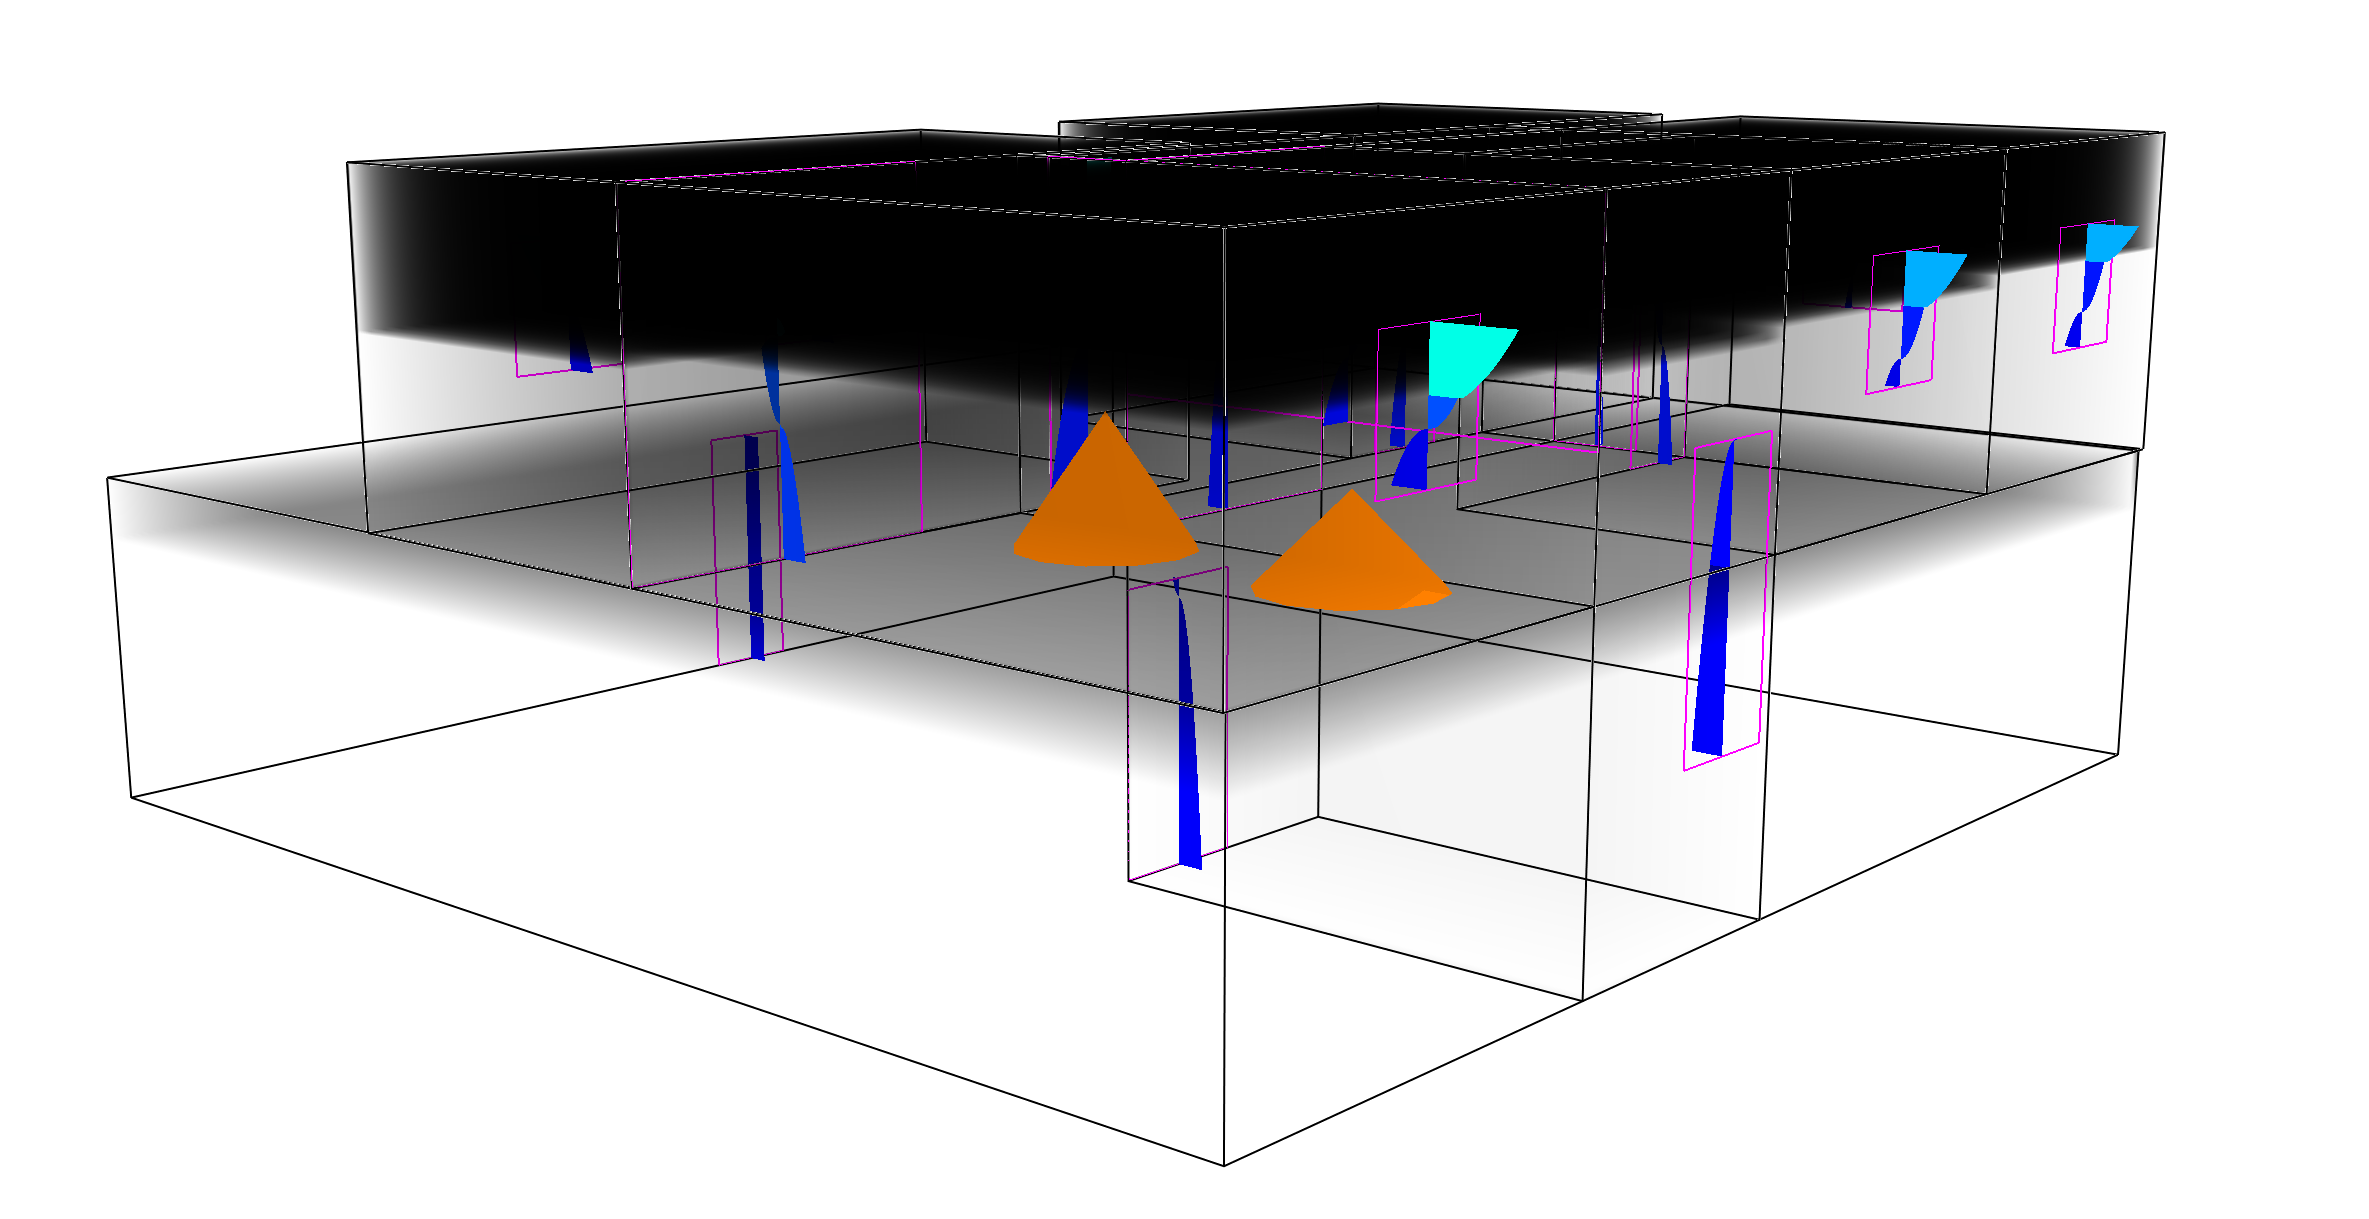
\includegraphics[width=4.5in]{FIGURES/Sample_Visualization.png}
\caption{Sample CFAST visualization of a single structure subject to a fire.}
\label{sample_visualization}
\end{figure}

Of course, if it is desired to study the impact of fires in a set of more than one specific building, the compartment geometry and placement could be defined by multiple individual buildings with the specific building chosen for an individual scenario chosen at random or from a distribution representing the population of each building type in the community under study.

The set of buildings for study can also be chosen from distributions of building and room characteristics. Figure \ref{sample_room_distribution} shows the distribution of the total floor area in a residence, the number of bedrooms in a residence depending on the total floor area, the total number of rooms given a certain number of bedrooms (here shown for residences from 1000~ft$^2$ to 1500~ft$^2$), all taken from the 2015 U.S. Housing Survey \cite{AHS2015}. Creating a compartment geometry from these data can be thought of as a six step process:

\begin{enumerate}
    \item randomly select the total floor area of the structure, Fig. \ref{sample_room_distribution}(a);
    \item randomly select the total number of bedrooms for a structure of the size chosen in step 1, Fig. \ref{sample_room_distribution}(b);
    \item randomly select the total number of rooms in the structure of the chosen size and number of bedrooms (Fig. \ref{sample_room_distribution}(c) shows a sample distribution for homes ranging from 1000~ft$^2$ to 1500~ft$^2$. Distributions for other home sizes are available in ref. \cite{AHS2015});
    \item determine room sizes based on a distribution of bedroom sizes, allocating left over space to the other rooms;
    \item connect compartments as desired (for example by randomly setting vents as open or closed between compartment pairs); and
    \item ensure that the resulting structure is realizable (This random approach to generating connections has a probability of resulting in a floorplan that cannot be instantiated in a single story. More technically, if the floorplan is thought of as a graph with the rooms as vertices and the connections as edges, some of the randomly generated graphs will be nonplanar for cases with more than four rooms. A planar graph is one that can be drawn on a piece of paper and none of the edges cross. The probability of generating a nonplanar floorplan increases as the number of rooms increases. In order to eliminate such nonphysical cases from the analysis, any randomly generated floorplan can be checked for planarity and rejected if necessary and replaced by a new randomly generated floorplan).
\end{enumerate}

\begin{figure}[p]
\begin{tabular*}{\textwidth}{c}
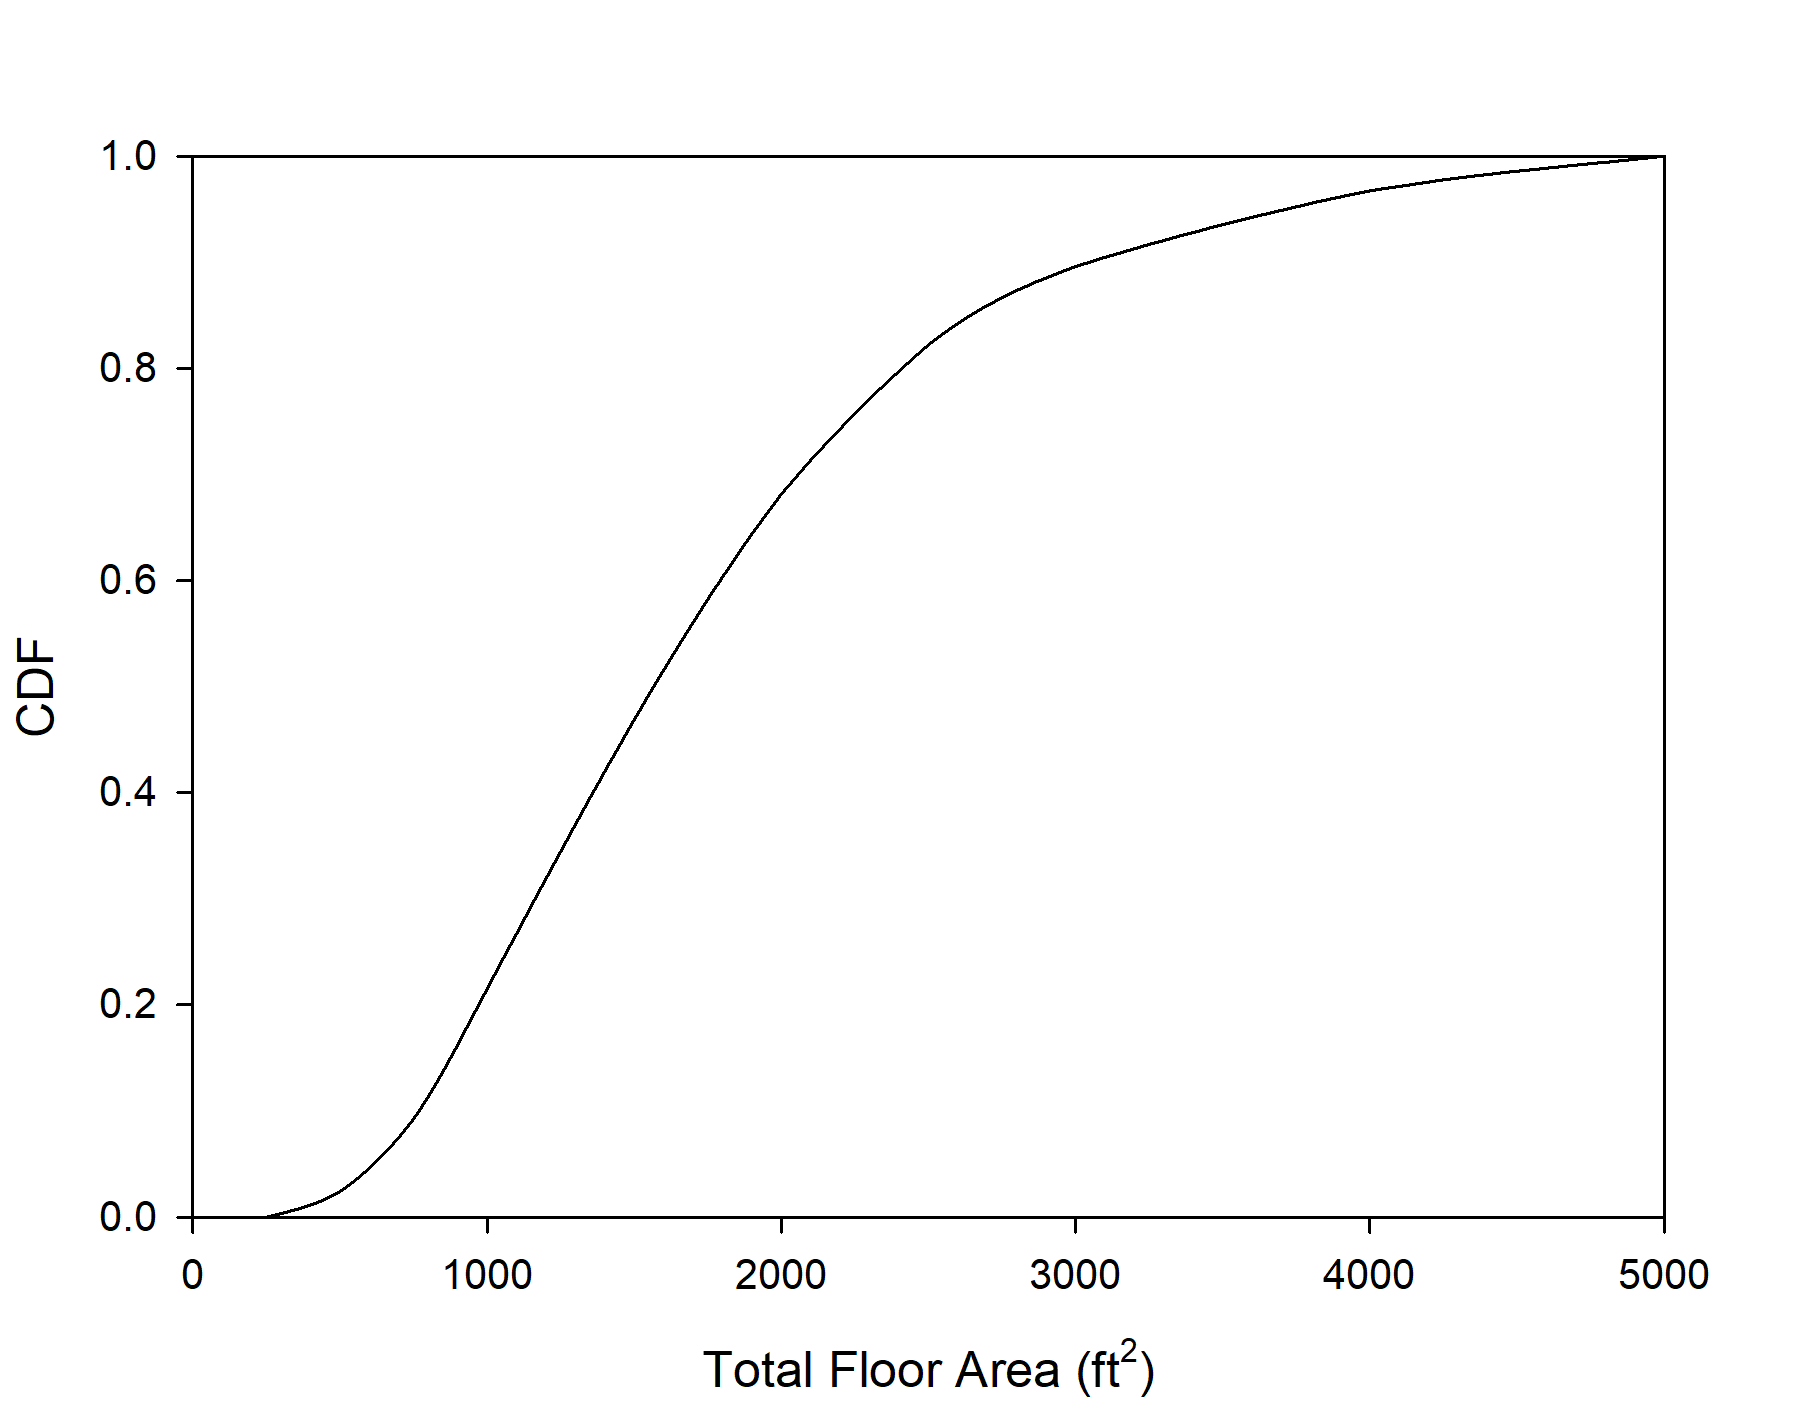
\includegraphics[height=2.5in]{FIGURES/Total_Floor_Area} \\
(a) Total Floor Area in a Residence \\
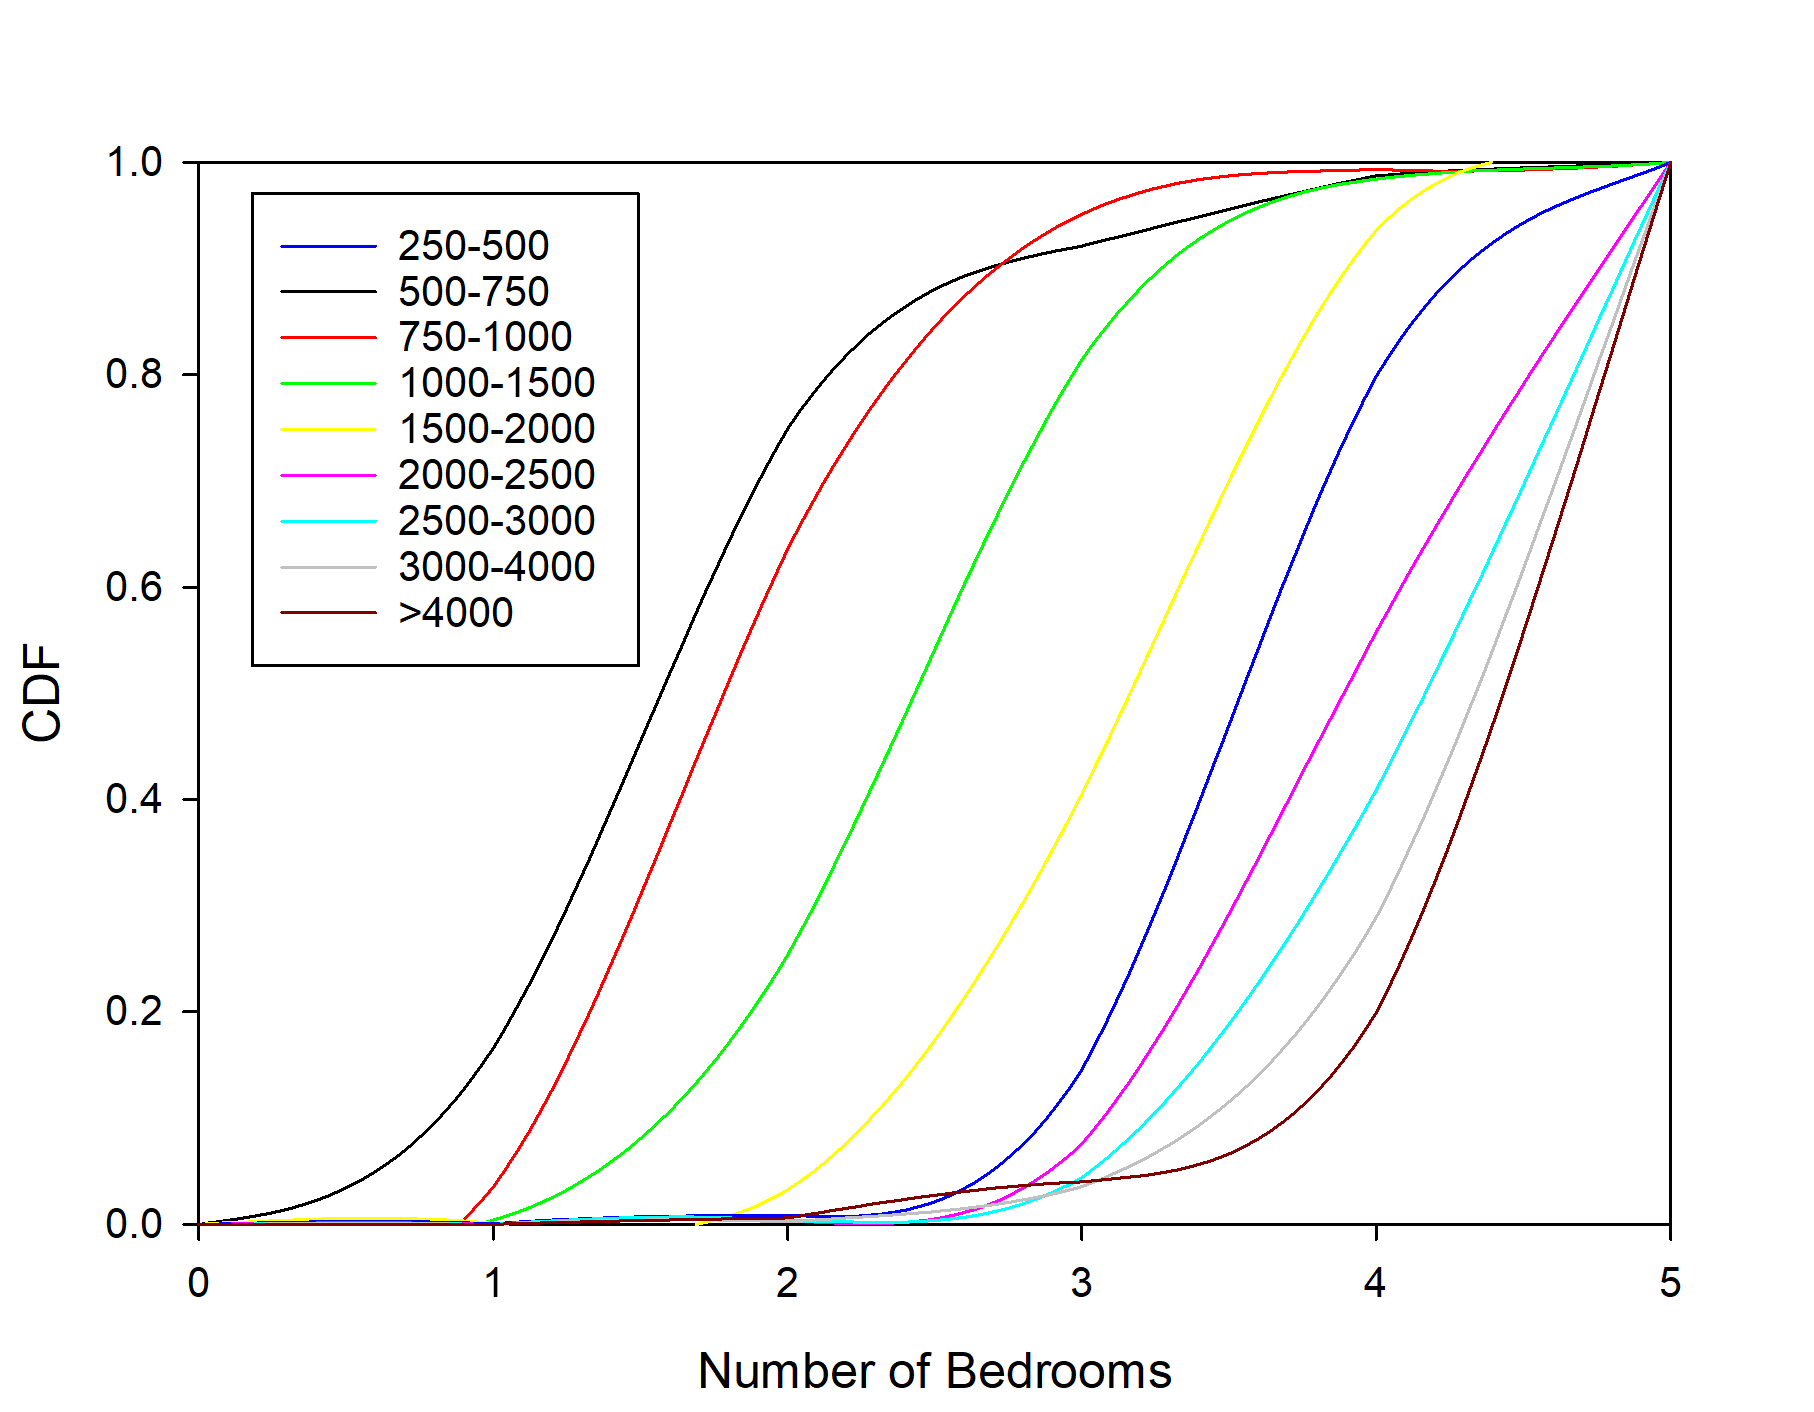
\includegraphics[height=2.5in]{FIGURES/Number_of_Bedrooms} \\
(b) Number of Bedrooms in a Residence as a Function of Total Floor Area \\
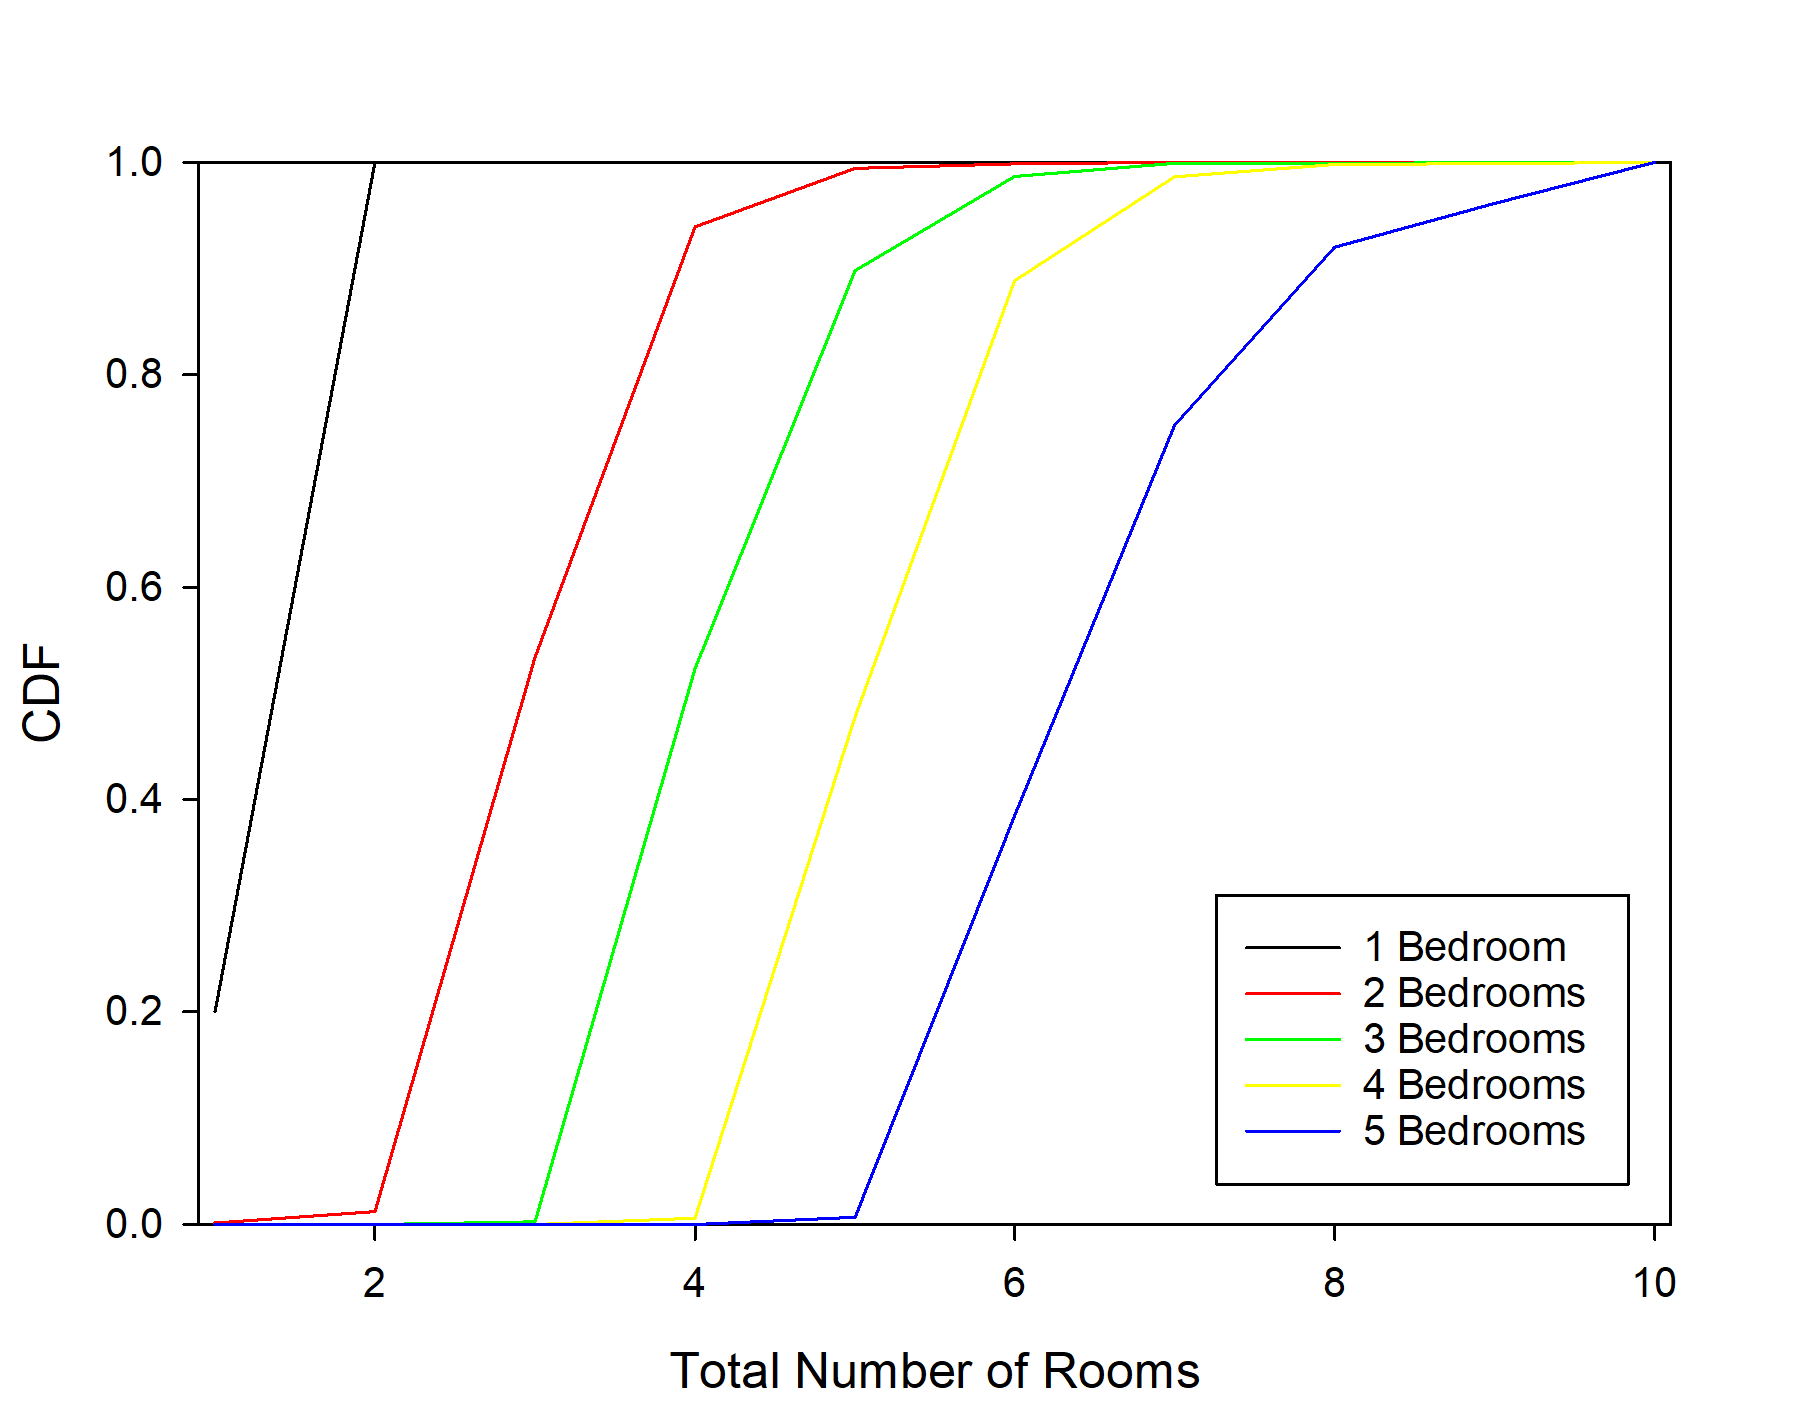
\includegraphics[height=2.5in]{FIGURES/Total_Rooms} \\
(c) Total Number of Rooms as a Function of the Number of Bedrooms in a Residence with  \\
1000 ft$^2$ - 1500 ft$^2$ of Total Floor Area  \\
\end{tabular*}
\caption[Cumulative Probability Distributions for Home Size, Number of Bedrooms and Total Number of Rooms]
{Example Cumulative Probability Distributions for Home Size, Number of Bedrooms and Total Number of Rooms (excluding Bathrooms) taken from the 2015 U.S. Housing Survey \cite{AHS2015}}
\label{sample_room_distribution}
\end{figure}

Other characteristics of the structure such as materials of construction, vent openings, fire definitions, measurement targets, sprinklers, and detection devices can be varied as desired for the problem being studied. Table \ref{tbl:distributable_variables} shows variables in the modeling that can be varied based on user-defined distributions \footnote{The content of this table follows the form of that used in B-Risk \cite{BranzFire}, adapted to be applicable to the calculational capabilities of the CFAST model.}.

\noindent
\begin{longtable}{@{\extracolsep{\fill}}|l|l|l|}
\caption[CFAST Inputs That Can be Varied Based on User-Defined Distributions]{CFAST Inputs That Can be Varied Based on User-Defined Distributions}
\label{tbl:distributable_variables} \\ \hline
\parbox{2in}{\bf Category}    & \parbox{2in}{\bf Input}  & \parbox{2in}{\bf Units} \\ \hline
\endfirsthead
\caption[]{Continued} \\ \hline
\parbox{2in}{\bf Category}    & \parbox{2in}{\bf Input}  & \parbox{2in}{\bf Units} \\ \hline
\endhead
Ambient Conditions      & Interior Temperature          & \degc                     \\
                        & Exterior Temperature          & \degc                     \\
                        & Relative Humidity             & \%                        \\ \hline
Thermal Properties      & Thermal Conductivity          & kW/(m~\degc)              \\
                        & Specific Heat                 & kJ/(kg~\degc)             \\
                        & Density                       & kg/m$^3$                  \\
                        & Default Thickness             & m                         \\
                        & Emissivity                    &                           \\ \hline
Compartments            & Width                         & m                         \\
                        & Depth                         & m                         \\
                        & Height                        & m                         \\
                        & Width Position                & m                         \\
                        & Depth Position                & m                         \\
                        & Height Position               & m                         \\
                        & Wall Leak Area Ratio          & m$^2$/m$^2$               \\
                        & Floor Leak Area Ratio         & m$^2$/m$^2$               \\ \hline
 Wall Vents             & Sill                          & m                         \\
                        & Soffit                        & m                         \\
                        & Width                         & m                         \\
                        & Initial Opening Fraction      & 0-1                       \\
                        & Open/Close Time               & s                         \\
                        & Final Opening Fraction        & 0-1                       \\
                        & Setpoint                      & s, \degc, or kW/m$^2$     \\
                        & Pre-Activation Fraction       & 0-1                       \\
                        & Post-Activation Fraction      & 0-1                       \\ \hline
 Ceiling / Floor Vents  & Cross-Sectional Area          & m$^2$                     \\
                        & Initial Opening Fraction      & 0-1                       \\
                        & Open/Close Time               & s                         \\
                        & Final Opening Fraction        & 0-1                       \\
                        & Setpoint                      & s, \degc, or kW/m$^2$     \\
                        & Pre-Activation Fraction       & 0-1                       \\ \hline
 Mechanical Vents       & From Compartment Area         & m$^2$                     \\
                        & From Compartment Height       & m                         \\
                        & To Compartment Area           & m$^2$                     \\
                        & To Compartment Height         & m                         \\
                        & Flow Rate                     & m$^3$/s                   \\
                        & Begin Dropoff                 & Pa                        \\
                        & End Dropoff                   & Pa                        \\
                        & Initial Opening Fraction      & 0-1                       \\
                        & Open/Close Time               & s                         \\
                        & Final Opening Fraction        & 0-1                       \\
                        & Setpoint                      & s, \degc, or kW/m$^2$     \\
                        & Pre-Activation Fraction       & 0-1                       \\
                        & Post-Activation Fraction      & 0-1                       \\
                        & Filter Efficiency             & \%                        \\
                        & Begin Filtering Time          & s                         \\ \hline
Fires                   & \multicolumn{2}{|c|}{See Section \ref{Fire_Scenarios}}    \\ \hline
Targets                 & Width Target Position         & m                         \\
                        & Depth Target Position         & m                         \\
                        & Height Target Position        & m                         \\
                        & Width Normal Vector           & 0-1                       \\
                        & Depth Normal Vector           & 0-1                       \\
                        & Height Normal Vector          & 0-1                       \\
                        & Target Points To              & Selection List            \\
                        & Thickness                     & m                         \\
                        & Internal Temperature Location & m                         \\ \hline
Detection / Suppression & Width Position                & m                         \\
                        & Depth Position                & m                         \\
                        & Height Position               & m                         \\
                        & Activation Temperature        & \degc                     \\
                        & Activation Obscuration        & \%/m                      \\
                        & RTI                           & (m~s)$^{1/2}$             \\
                        & Spray Density                 & m/s                       \\ \hline
\end{longtable}

\clearpage

\section{Fire Scenarios}
\label{Fire_Scenarios}

\subsection{Individual Variables}

The quantitative definition of fires is arguably the most important \cite{Babrauskas:1992} and complex of all the inputs in any fire modeling scenario. It includes specification of the fire location, fuel composition, ignition criterion, heat release rate, burning area, and species yields, most of which can vary with time over the course of the fire.

\noindent
\begin{longtable}{@{\extracolsep{\fill}}|l|l|l|}
\caption[CFAST Fire Inputs That Can be Varied Based on User-Defined Distributions]{CFAST Fire Inputs That Can be Varied Based on User-Defined Distributions}
\label{tbl:fire_variables} \\ \hline
\parbox{2in}{\bf Category}    & \parbox{2in}{\bf Input}  & \parbox{2in}{\bf Units} \\ \hline
\endfirsthead
\caption[]{Continued} \\ \hline
\parbox{2in}{\bf Category}    & \parbox{2in}{\bf Input}  & \parbox{2in}{\bf Units} \\ \hline
\endhead
Fire Location           & Compartment                   & Selection List                \\
                        & Width Position                & m                             \\
                        & Depth Position                & m                             \\ \hline
Fuel Composition        & Carbon Molecules              & $\geq$ 0                      \\
                        & Hydrogen Molecules            & $\geq$ 0                      \\
                        & Oxygen Molecules              & $\geq$ 0                      \\
                        & Nitrogen Molecules            & $\geq$ 0                      \\
                        & Chlorine Molecules            & $\geq$ 0                      \\
                        & Heat of Combustion            & kJ/kg                         \\
                        & Radiative Fraction            & 0 - 1                         \\ \hline
Ignition Criteria       & Ignition Criterion            & Selection List                \\
                        & Setpoint                      & s, \degc, or kW/m$^2$         \\ \hline
Time Histories          & \multicolumn{2}{|c|}{See Section \ref{Fire_Time_Histories}}   \\ \hline
\end{longtable}

\subsection{Time Histories}
\label{Fire_Time_Histories}

Some examples of different definitions of time histories go here.

\noindent
\begin{longtable}{@{\extracolsep{\fill}}|l|l|l|}
\caption[CFAST Fire Time Histories That Can be Varied Based on One or More User-Defined Distributions]{CFAST Fire Time Histories That Can be Varied Based on One or More User-Defined Distributions}
\label{tbl:fire_variables} \\ \hline
\parbox{2in}{\bf Category}    & \parbox{2in}{\bf Input}  & \parbox{2in}{\bf Units} \\ \hline
\endfirsthead
\caption[]{Continued} \\ \hline
\parbox{2in}{\bf Category}    & \parbox{2in}{\bf Input}  & \parbox{2in}{\bf Units} \\ \hline
\endhead
Time Histories          & HRR                           & kW                        \\
                        & Fire Height                   & m                         \\
                        & Fire Area                     & m$^2$, >0                 \\
                        & CO Yield                      & kg CO/kg fuel             \\
                        & Soot Yield                    & kg Soot/kg fuel           \\
                        & HCN Yield                     & kg HCN/kg fuel            \\ \hline
\end{longtable}

\section{Defining Data for Analysis}
\label{commands_section}

Choosing modeling results for analysis depends on the goals of the hazard analysis and the particular technology under study. In the most general sense, this means understanding what results are indicative of improved fire safety. This is not a cost benefit analysis, which is a superset of this analysis and outside the scope of this project. To improve fire safety generally means reducing the deaths and injuries due to a fire. So, the goal is to identify which variables, that can be calculated, would give an indication that a new technology will reduce deaths and injuries.

Each subsection will discuss one set of namelist inputs and what each of the parameters do. All the inputs are combined in Appendix \ref{preprocessor_reference}  to serve as a reference for commands.

\subsection{Namelist MHDR}

The {\ct \&MHDR} inputs specify details of the scenarios to be generated including the number of cases to be generated, seeds for the random number generator, and locations for input and output files.

\begin{description}
  \item[NUMBER\_OF\_CASES] (default value 1): specifies the number of cases that the preprocessor will generate.
  \item[RANDOM\_SEEDS] (default value, software chosen random integer pair): defines an integer pair used to determine random number seeds for distributions. Any two integers (excluding -1001 which is used internally to indicate default values) may be specified. Including random seeds here will ensure that the same cases will be generated each time the preprocessor is run for a given input file. Changing the random seeds (or other inputs) will result in a different set of input files.  All seeds are written in the {\ct <project>\_seeds.csv} file, if specified.
  \item[WRITE\_RANDOM\_SEEDS] (default value, .TRUE.): if .TRUE., all random number seeds are saved in the file {\ct <project>\_seeds.csv}.
  \item[PARAMETER\_FILE] (default value, {\ct <project>\_parameters.csv} where {\ct <project>} is the base filename of the CDATA/CFAST input file): Summary output file from the preprocessor that list the CFAST file names and parameter values for inputs varied for each CFAST scenario in the set of generated CFAST cases. This file is combined with the summary statistics generated by the accumulator module.
  \item[WORK\_FOLDER] (default value, current folder): folder where the preprocessor creates its set of CFAST inputs file and where the accumulator looks for CFAST output files to be processed.
  \item[OUTPUT\_FOLDER] (default value, current folder): folder where the accumulator or statistics modules put their output files of analysis results.
\end{description}

\vspace{\baselineskip}
\noindent Examples:
\begin{lstlisting}
&MHDR NUMBER_OF_CASES = 10000 /
&MHDR NUMBER_OF_CASES = 20000 WRITE_SEEDS = .TRUE.
	PARAMETER_FILE = 'Outputfile' WORK_FOLDER = 'Z:\'  OUTPUT_FOLDER = '..\project'/
\end{lstlisting}



\subsection{Namelist MRND}

The {\ct \&MRND} defines a random number generator that uses a number of inputs to specify distributions for variation. A generator specifies a single random variable for each case so that every input using a particular generator will get the same value for each case. In the simplest cases every field that a user wants to vary will require a separate random generator. However, suppose the desire is to have all the rooms have the same height ceiling, then all the fields will use the same random number generator. % This might be to early to say all this. What do you think?

\begin{description}
  \item[ID] Distributions are defined by a unique alphanumeric name. This may be as simple as a single character or number, or a description of the distribution. All IDs must be unique throughout an input file.
  \item[FYI] A user defined comment that can provide additional information about the input.
  \item[TYPE] identifies the type of distribution. Additional required inputs depend of the type of distribution defined. Allowed distributions are {\ct CONSTANT},  {\ct UNIFORM}, {\ct TRIANGLE}, {\ct NORMAL}, {\ct LOG\_NORMAL}, {\ct BETA}, {\ct LINEAR }, and {\ct USER\_DEFINED}.
  \item[RANDOM\_SEEDS] like {\ct RANDOM\_SEEDS} in {\ct \&MHDR}, an integer pair specifies initial seeds for the random number generator, but applies only to the specific distribution. Any two integers (excluding -1001 which is used internally to indicate default values) may be specified. Including random seeds here will ensure that the same cases will be generated each time the preprocessor is run for a given input file. Changing the random seeds (or other inputs) will result in a different set of input files. All seeds are written in the {\ct <project>\_seeds.csv} file, if specified.
  \item[VALUES] a set of values for the {\ct USER\_DEFINED} distribution type. Inputs are input as string constants and interpreted to match the type required by the associated {\ct \&MRND} input(s). Values for an individual scenario are chosen randomly from the list of values provided.
  \item[PROBABILITIES] a set of probabilities values for the {\ct USER\_DEFINED} distribution type. These are not cumulative probabilities and the total of all values must add to 1.0
  \item[CONSTANT] is a constant value. For the {\ct CONSTANT} distribution it is the value that is returned by the generator.
  \item[MINIMUM] minimum value for the {\ct UNIFORM}, {\ct TRIANGLE}, and {\ct LINEAR} distribution types.
  \item[MAXIMUM] maximum value for the {\ct UNIFORM}, {\ct TRIANGLE}, and {\ct LINEAR} distribution types.
  \item[PEAK] peak value for the {\ct TRIANGLE} distribution type.
  \item[ALPHA] alpha value for the {\ct BETA} distribution type.
  \item[BETA] beta value for the {\ct BETA} distribution type.
  \item[MEAN] mean value for the {\ct NORMAL}; geometric mean value for the {\ct LOG\_NORMAL} distribution type.
  \item[STDEV] standard deviation value for the {\ct NORMAL}; geometric standard deviation value for the {\ct LOG\_NORMAL} distribution type.
  \item[MINIMUM\_FIELD] specifies the name of the specific input (i.e., the name of a compartment, vent, etc.) and the specific field within that input that is to be taken as the minimum value of the distribution returned. It allows the range to be defined by another input. For example, if the {\ct \&MRND} input is used to vary the ceiling height the top of a vent can be used as the lowest value for the ceiling height by including a {\ct MINIMUM\_FIELD} input for the compartment height input such as {\ct MINIMUM\_FIELD="Vent 1", "TOP"} to limit how low height of the compartment is set.
  \item[MAXIMUM\_FIELD] specifies the name of the specific input (i.e., the name of a compartment, vent, etc.) and the specific field within that input that is to be taken as the maximum value of the distribution returned. It allows the range to be defined by another input. For example, if the {\ct \&MRND} input is used to vary the top of a vent, then you can set the upper limit the height in the associated compartment by including a {\ct MAXIMUM\_FIELD} input for the vent input such as {\ct MAXIMUM\_FIELD="Comp 1","HEIGHT"} to cap the vent top to the height of the compartment.
\end{description}

\vspace{\baselineskip}
\noindent Example:
\begin{lstlisting}
&MRND ID = 'Example rand generator', TYPE = 'UNIFORM',  MINIMUM = 10, MAXIMUM = 50 /
&MRND ID ='Second rand generator', TYPE = 'NORMAL', MEAN = 0, STDEV = 1 /
\end{lstlisting}

\subsection{Namelist MFLD}

\begin{description}
  \item[ID] Varied input fields are defined by a unique alphanumeric name. This may be as simple as a single character or number, or a description of the field. All IDs must be unique throughout an input file.
  \item[FYI] A user defined comment that can provide additional information about the input.
  \item[FIELD] specifies the name of the specific input (i.e., the name of a compartment, vent, etc.) and the specific field within that input that is to be varied. For example, {\ct FIELD="Comp 1","HEIGHT"} would vary the height of the compartment named {\ct Comp 1}.
  \item[TYPE] specifies the type of field data used to fill in values in the specified field. Additional inputs depend on the type of field specified. Allowed field types are {\ct VALUE}, {\ct SCALING}, {\ct LABEL}, and {\ct INDEX}. {\ct VALUE} simply takes the value returned from the specified random generator and places it directly in the specified field. {\ct SCALING} takes the returned value and multiplies by the {\ct BASE\_SCALING\_VALUE} and puts that value in the field. {\ct INDEX} requires the random generator to return integers as an index into the {\ct VALUES} input (starting at 1 to the number of inputs in the {\ct VALUES}       input for the current {\ct \&MFLD} input). The value in the {\ct INDEX\_TYPE}, {\ct REAL}, {\ct INTEGER}, {\ct CHARACTER}, or {\ct LOGICAL}, array at the index is placed in the field.
  \item[FIELD\_LABELS] The purpose of this optional is simply to provide descriptions of the purpose of each index value for {\ct INDEX} inputs.
  \item[RAND\_ID] specifies the ID of associated {\ct \&MRND} input used to provide random inputs for the field. These may be unique to each field input or more than one field input may use the same {\ct \&MRND} input to coordinate values for multiple input fields. The number of inputs in the {\ct \&MRND} input must match those for the field type.
  \item[ADD\_TO\_PARAMETERS] set to .TRUE. to include the value of the field in the parameters file, {\ct <project>\_parameters.csv}. Default value is .TRUE.
  \item[PARAMETER\_COLUMN\_LABEL] specifies the column title for this input field in the parameters file, {\ct <project>\_parameters.csv}. If it is not included CData will use a combination of the {\ct FIELD} inputs to create a column label.
  \item[VALUES] a set of values for the {\ct INDEX} field type. Values for an individual scenario are chosen randomly from the list of values provided. The type of the inputs is determined by the type of value needed from the {\ct FIELD} input but all inputs in the {\ct VALUES} inputs are specified in a character array input.
  \item[BASE\_SCALING\_VALUE] Initial value of the field for the {\ct SCALING} type field. Defaults to the value in the base input file if not included.
\end{description}

\vspace{\baselineskip}
\noindent Example:

The following example shows the height of the bedroom varying uniformly from 2.44 m to 3.66 m.
\begin{lstlisting}
&MRND ID = 'Room height generator', TYPE = 'UNIFORM',  MINIMUM = 2.44, MAXIMUM = 3.66 /
&MFLD ID = 'Height bedroom' FIELD = 'Bedroom', 'HEIGHT' RAND_ID = 'Room height generator' PARAMETER_COLUMN_LABEL = 'Bedroom height' /
\end{lstlisting}

The following example shows the height of a door to the bedroom in the above example varying from a minimum of 2 m to a maximum 0.15 m below the ceiling of the varying height of the bedroom ceiling.

\begin{lstlisting}
&MRND ID = 'Door Top Generator' DISTRIBUTION_TYPE = 'UNIFORM' VALUE_TYPE = 'REAL'
    MINIMUM = 2.0 MAXIMUM_FIELD = 'Height Bedroom' MAXIMUM_OFFSET = -0.15 /
&MFLD ID = 'Door Top' FIELD_TYPE = 'VALUE' RAND_ID = 'Door Top Generator' FIELD = 'Wall Vent' 'TOP' /
\end{lstlisting}


\clearpage

\subsection{Namelist MFIR}

Automatically-generated fires are created for an individual test case by modifying an existing fire input in the input file. The {\ct \&MFIR} input allows the user to either scale the HRR curve (multiplying the time and/or HRR values by a constant defined by a user-specified distribution) or by defining a power law fire based on several inputs.

\begin{description}
  \item[ID] All inputs are defined by a unique alphanumeric name. This may be as simple as a single character or number, or a description of the field. All IDs must be unique throughout an input file.
  \item[FYI] A user defined comment that can provide additional information about the input.
  \item[FIRE\_ID] Specifies the associated fire in the data file that is used as a template to be modified by this {\ct \&MFIR} input. All inputs in the current {\ct \&MFIR} namelist will modify this fire.
  \item[MODIFY\_FIRE\_AREA\_TO\_MATCH\_HRR] IF set to {\ct .TRUE.}, the fire area is calculated from the heat release rate values for the time curve from the formula. Values are calculated from heat release rate such that the fire Froude number is unity\footnote{The Fire Froude Number, $\dQ^*$, is defined as $\dQ^* = \frac{\dQ}{\rho_\infty c_p T_\infty \sqrt{gD} D^2}$. It is essentially the ratio of the fuel gas exit velocity and the buoyancy-induced plume velocity. Jet fires are characterized by large Froude numbers. Typical accidental fires have a Froude number near unity.}.
  \item[FIRE\_COMPARTMENT\_RANDOM\_GENERATOR\_ID] A random generator that returns an index to pick the compartment the fire is located. Usually uses {\ct USER\_DEFINED\_DISCRETE\_DISTRIBUTION}.
  \item[FIRE\_COMPARTMENT\_IDS] A list of compartment names that have a chance of having the fire in them. This matches the index chosen by {\ct FIRE\_COMPARTMENT\_RANDOM\_GENERATOR\_ID} to actual compartment names in the input file.
  \item[ADD\_FIRE\_COMPARTMENT\_ID\_TO\_PARAMETERS] set to .TRUE. to include the value of the field in the parameters file, {\ct <project>\_parameters.csv}. Default value is .TRUE.
  \item[FIRE\_COMPARTMENT\_ID\_COLUMN\_LABEL] specifies the column title for this input field in the parameters file, {\ct <project>\_parameters.csv}. If it is not included, it will be filled in by the code.
  \end{description}
Fires can be defined by either scaling time and/or HRR values from a base fire or by defining a power law fire growth / decay with a peak plateau period. Either fire can be proceeded by an optional period of incipient fire growth period. Firstly, the inputs for the incipient fire are described.

 \begin{description}
  \item[FLAMING\_SMOLDERING\_IGNITION\_DELAY\_RANDOM\_GENERATOR\_ID] This and the two entries {\ct INCIPIENT\_FIRE\_TYPES} and {\ct TYPE\_OF\_INCIPIENT\_GROWTH} work together. This one determines if you have a smoldering or flaming incipient fire. Ignition is not delayed, that is badly worded. If this one is not defined then only one of the two sets of two can be defined and the other two must not be left blank. This is a I{\ct INDEX} type of field because this gives the most flexibility
  \item[INCIPIENT\_FIRE\_TYPES] A list made up of 'FLAMING' and 'SMOLDERING'. This allows users to coordinate the incipient beginning of the fire with other inputs in the scenario.
  \item[TYPE\_OF\_INCIPIENT\_GROWTH] Defaults to {\ct NONE} but can be {\ct FLAMING}, {\ct SMOLDERING}, and {\ct RANDOM}
  \item[FLAMING\_IGNITION\_DELAY\_RANDOM\_GENERATOR\_ID] This is the first of the flaming set of generators and defines an associated {\ct \&MRND} ID that defines the length of the incipient flaming fire burning period. If you do not want the value to change you can set it up to a {\ct CONSTANT} random generator. If included, both {\ct FLAMING\_IGNITION\_DELAY\_RANDOM\_GENERATOR\_ID} and {\ct PEAK\_FLAMING\_IGNITION\_RANDOM\_GENERATOR\_ID} must be defined.
  \item[PEAK\_FLAMING\_IGNITION\_RANDOM\_GENERATOR\_ID] This is the second of the flaming set of generators and defines an associated {\ct \&MRND} ID that defines the final HRR for the incipient flaming fire ramp. If you do not want the value to change you can set it up to a {\ct CONSTANT} random generator. If included, both {\ct FLAMING\_IGNITION\_DELAY\_RANDOM\_GENERATOR\_ID} and {\ct PEAK\_FLAMING\_IGNITION\_RANDOM\_GENERATOR\_ID} must be defined. This one determines the final HRR for the flaming fire ramp. It is important to understand that using this means the first two HRR points will be overwritten and all times for all entries in the fire will be set to the same.
  \item[SMOLDERING\_IGNITION\_DELAY\_RANDOM\_GENERATOR\_ID] This is the smoldering pair that match the above.
  \item[PEAK\_SMOLDERING\_IGNITION\_RANDOM\_GENERATOR\_ID] Same as above for smoldering fire.
  \item[ADD\_IGNITION\_TYPE\_TO\_PARAMETERS] set to .TRUE. to include the value of the field in the parameters file, {\ct <project>\_parameters.csv}. Default value is .TRUE. Column displays 'FLAMING' or 'SMOLDERING' depending on which type of ignition happens.
  \item[ADD\_SMOLDERING\_IGNITION\_TIME\_TO\_PARAMETERS] set to .TRUE. to include the value of the field in the parameters file, {\ct <project>\_parameters.csv}. Default value is .TRUE.
  \item[ADD\_SMOLDER\_IGNTION\_PEAK\_TO\_PARAMETERS] Name shortened because adding the 'ING' made the variable name too long and it got truncated. Defaults to {\ct .TRUE.}
  \item[ADD\_FLAMING\_IGNTION\_TIME\_TO\_PARAMETERS] set to .TRUE. to include the value of the field in the parameters file, {\ct <project>\_parameters.csv}. Default value is .TRUE.
  \item[ADD\_FLAMING\_IGNITION\_PEAK\_HRR\_TO\_PARAMETERS] set to .TRUE. to include the value of the field in the parameters file, {\ct <project>\_parameters.csv}. Default value is .TRUE.
  \item[FLAMING\_HRR\_PEAK\_COLUMN\_LABEL] specifies the column title for this input field in the parameters file, {\ct <project>\_parameters.csv}. If it is not included, it will be filled in by the code.
  \item[FLAMING\_TIME\_COLUMN\_LABEL] specifies the column title for this input field in the parameters file, {\ct <project>\_parameters.csv}. If it is not included, it will be filled in by the code.
  \item[SMOLDERING\_HRR\_PEAK\_COLUMN\_LABEL] specifies the column title for this input field in the parameters file, {\ct <project>\_parameters.csv}. If it is not included, it will be filled in by the code.
  \item[SMOLDERING\_TIME\_COLUMN\_LABEL] specifies the column title for this input field in the parameters file, {\ct <project>\_parameters.csv}. If it is not included, it will be filled in by the code.
 \end{description}
Secondly, inputs for the scaling fire are described.

\begin{description}
  \item[BASE\_FIRE\_ID] For scaling fires only. This provides internal temporary storage for all the base values for a fire to be scaled. Typically, it will just be a copy of the corresponding {\ct FIRE\_ID} input.
  \item[SCALING\_FIRE\_HRR\_RANDOM\_GENERATOR\_ID] an associated {\ct \&MRND} ID that defines the scaling factor that is applied to all the HRR values in a fire. This is done before the incipient fire model is calculated so it won’t impact the delay or HRR value for the incipient fire portion of the fire curve.
  \item[SCALING\_FIRE\_TIME\_RANDOM\_GENERATOR\_ID] an associated {\ct \&MRND} ID that defines the  scaling value that is applied to all the TIME values in a fire. This is done before the Incipient fire model is calculated so it won’t impact the delay or HRR value for the incipient portion of the fire curve.
  \item[ADD\_HRR\_SCALE\_TO\_PARAMETERS] set to .TRUE. to include the value of the field in the parameters file, {\ct <project>\_parameters.csv}. Default value is .TRUE.
  \item[HRR\_SCALE\_COLUMN\_LABEL] specifies the column title for this input field in the parameters file, {\ct <project>\_parameters.csv}. If it is not included, it will be filled in by the code.
  \item[ADD\_TIME\_SCALE\_TO\_PARAMETERS] set to .TRUE. to include the value of the field in the parameters file, {\ct <project>\_parameters.csv}. Default value is .TRUE.
  \item[TIME\_SCALE\_COLUMN\_LABEL] specifies the column title for this input field in the parameters file, {\ct <project>\_parameters.csv}. If it is not included, it will be filled in by the code.
  \end{description}
  Finally, the inputs for a general power law fire are described. The calculation of the growth and decay points is straightforward enough. The inputs are $t_0$, $t_1$, $\dQ_0$, $\dQ_1$, and the exponential growth $r$. The variables $t_0$ and $t_1$ are the beginning and ending time points and $\dQ_0$ and $\dQ_1$ are the HRR at the beginning and end and $r$ is already defined. For growth $\hat{t} = t + t_0$ where $0<t<t_1 - t_0$ and for decay $\hat{t} = t_1 - t$ where $0<t<t_1 - t_0$. The equation for the HRR at time $t$ in the growth phase is $\dQ(\hat{t}) = ((\dQ_1 - \dQ_0)/(t_1-t_0)^r)\hat{t} + \dQ_0$ and for decay is $\dQ(\hat{t}) = ((\dQ_0 - \dQ_1)/(t_1-t_0)^r)\hat{t} + \dQ_1$. It can be done based on which, $\dQ_0$ or $\dQ_1$, are larger.

\begin{description}
  \item[FIRE\_TIME\_GENERATORS] a set of up to 100 associated {\ct \&MRND} inputs that define the time intervals for fire growth If you do not want the values to change you can set any of the {\ct \&MRND} inputs to a {\ct CONSTANT} random generator. The first point is always at $t=0$ and $\dQ = 0$. If there is an incipient fire defined, that is point two. If there is a power law growth defined (by {\ct GROWTH\_EXPONENT} and {\ct GROWTH\_EXPONENT}, these follow the first or second time point (depending on whether there is an incipient fire defined). If a power law decay is defined (by {\ct DECAY\_EXPONENT} and {\ct DECAY\_EXPONENT}, these are defined by the next to last and last generators defined.
  \item[FIRE\_HRR\_GENERATORS] a set of up to 100 associated {\ct \&MRND} inputs that define the HRR values corresponding with each defined time generator. If you do not want the values to change you can set any of the {\ct \&MRND} inputs to a {\ct CONSTANT} random generator.
  \item[NUMBER\_OF\_GROWTH\_POINTS] specifies the number of data points included in the growth phase of the fire.
  \item[NUMBER\_OF\_DECAY\_POINTS] specifies the number of data points included in the decay phase of the fire.
  \item[GROWTH\_EXPONENT]  specifies the exponent of the power law for the growth phase of the fire.
  \item[DECAY\_EXPONENT] specifies the exponent of the power law for the decay phase of the fire.

  \item[ADD\_HRR\_TO\_PARAMETERS] set to .TRUE. to include the value of the field in the parameters file, {\ct <project>\_parameters.csv}. Default value is .TRUE.
  \item[ADD\_TIME\_TO\_PARAMETERS] set to .TRUE. to include the value of the field in the parameters file, {\ct <project>\_parameters.csv}. Default value is .TRUE.
  \item[TIME\_COLUMN\_LABEL] specifies the column title for this input field in the parameters file, {\ct <project>\_parameters.csv}. If it is not included, it will be filled in by the code.
  \item[HRR\_COLUMN\_LABEL] specifies the column title for this input field in the parameters file, {\ct <project>\_parameters.csv}. If it is not included, it will be filled in by the code.
\end{description}

\vspace{\baselineskip}
\noindent Example:
\begin{lstlisting}
&MRND ID = 'Generator for fire rooms' DISTRIBUTION_TYPE = 'USER_DEFINED_DISCRETE' VALUE_TYPE = 'INTEGER'
    INTEGER_VALUES = 1, 2, 3 PROBABILITIES = 0.3333 0.3333 0.3334 /
&MRND ID = 'Flaming Smoldering Generator' DISTRIBUTION_TYPE = 'USER_DEFINED_DISCRETE' VALUE_TYPE = 'INTEGER'
    INTEGER_VALUES = 1 2 PROBABILITIES = 0.5 0.5 /
&MRND ID = 'Flaming Time Generator' DISTRIBUTION_TYPE = 'TRUNCATED_NORMAL' VALUE_TYPE = 'REAL' MEAN = 207 STDEV = 46
    MINIMUM = 10 MAXIMUM = 1000000/
&MRND ID = 'Flaming Peak Generator' DISTRIBUTION_TYPE = 'TRUNCATED_NORMAL' VALUE_TYPE = 'REAL' MEAN = 23000 STDEV = 7000
    MINIMUM = 100 MAXIMUM = 1000000/
&MRND ID = 'Smoldering Time Generator' DISTRIBUTION_TYPE = 'TRUNCATED_NORMAL' VALUE_TYPE = 'REAL' MEAN = 6863 STDEV = 1812
    MINIMUM = 60 MAXIMUM = 14490/
&MRND ID = 'Smoldering Peak Generator' DISTRIBUTION_TYPE = 'TRUNCATED_NORMAL' VALUE_TYPE = 'REAL' MEAN = 11000 STDEV = 3000
    MINIMUM = 100 MAXIMUM = 1000000/
&MRND ID = 'Growth Time  Generator', DISTRIBUTION_TYPE = 'TRUNCATED_NORMAL' VALUE_TYPE = 'REAL' MEAN = 205, STDEV = 65
    MINIMUM = 75 MAXIMUM = 500 /
&MRND ID = 'Peak HRR Generator', DISTRIBUTION_TYPE = 'CONSTANT' VALUE_TYPE = 'REAL' REAL_CONSTANT_VALUE = 1054000 /
&MRND ID = 'Peak Plateau End Time' DISTRIBUTION_TYPE = 'CONSTANT' VALUE_TYPE = 'REAL' REAL_CONSTANT_VALUE = 10 /
&MRND ID = 'Fire End Time' DISTRIBUTION_TYPE = 'CONSTANT' VALUE_TYPE = 'REAL' REAL_CONSTANT_VALUE = 10 /
&MRND ID = 'Fire End HRR' DISTRIBUTION_TYPE = 'CONSTANT' VALUE_TYPE = 'REAL' REAL_CONSTANT_VALUE = 0 /

&MFIR ID = 'Fire Generator' FIRE_ID = 'Random'
    FIRE_COMPARTMENT_RANDOM_GENERATOR_ID = 'Generator for fire rooms'
    FIRE_COMPARTMENT_IDS = 'Dining Room', 'Kitchen', 'Living Room'
    FLAMING_SMOLDERING_IGNITION_RANDOM_GENERATOR_ID = 'Flaming Smoldering Generator' TYPE_OF_INCIPIENT_GROWTH = 'RANDOM'
    NUMBER_OF_INCIPIENT_FIRE_TYPES = 2 INCIPIENT_FIRE_TYPES = 'FLAMING' 'SMOLDERING'
    PEAK_FLAMING_IGNITION_RANDOM_GENERATOR_ID = 'Flaming Time Generator'
    FLAMING_IGNITION_DELAY_RANDOM_GENERATOR_ID = 'Flaming Peak Generator'
    PEAK_SMOLDERING_IGNITION_RANDOM_GENERATOR_ID = 'Smoldering Time Generator'
    SMOLDERING_IGNITION_DELAY_RANDOM_GENERATOR_ID = 'Smoldering Peak Generator'
    FIRE_TIME_GENERATORS = 'Growth Time Generator' 'Peak Plateau End Time' 'Fire End Time'
    FIRE_HRR_GENERATORS =  'Peak HRR Generator'    'Peak HRR Generator'    'Fire End HRR'
    NUMBER_OF_GROWTH_POINTS = 10 GROWTH_EXPONENT = 2 /
\end{lstlisting}

\subsection{Namelist MSTT}

\begin{description}
 \item[ID] All inputs are defined by a unique alphanumeric name. This may be as simple as a single character or number, or a description of the field. All IDs must be unique throughout an input file.
  \item[FYI] A user defined comment that can provide additional information about the input.
 \item[ANALYSIS\_TYPE] Describes the type of analsysi to be done. The allowed types are {\ct HISTOGRAM}, {\ct EMPERICAL\_PDF}, {\ct CONVERGENCE\_OF\_MEAN}, and {\ct CORRELATION\_TREES}.
 \item[INPUT\_FILENAME] Comma delimited file that contains the data. The default is the {\ct input filename\_accumulate.csv}.
 \item[OUTPUT\_FILENAME] The file that the finish grafic should be named. The extension is required as that is the method of determine the format of the file. The accepted formats are {\ct *.jpg}, {\ct *.svg}, {\ct *.tif}, {\ct *.pdf}, {\ct *.png}.
 \item[ERROR\_FILENAME] Error filename defaults to {\ct OUTPUT\_FILENAME} with {\ct err} extension by default
 \item[LOG\_FILENAME] Log filename defaults to {\ct OUTPUT\_FILENAME} with {\ct log} extension by default
 \item[COLUMN\_TITLE] The name in the first row for the column to use for the analysis. 
\end{description}

\vspace{\baselineskip}
\noindent Example:
\begin{lstlisting}
&MSTT ID = 'Width of Vent' ANALYSIS_TYPE = 'HISTOGRAM' OUTPUT_FILENAME = 'simple_width.jpg' 
	COLUMN_TITLE = 'Wall Vent_WIDTH' /
&MSTT ID = 'Top of Vent' ANALYSIS_TYPE = 'HISTOGRAM' OUTPUT_FILENAME = 'simple_top.jpg' 
	COLUMN_TITLE = 'Wall Vent_TOP' /
\end{lstlisting}



\subsection{Namelist DUMP}

\begin{description}
  \item[ID] Summary outputs are defined by a unique alphanumeric name. The ID is not only used to identify the output but is also the column label for the output. This may be as simple as a single character or number, or a description of the output. All IDs must be unique throughout an input file.
  \item[FYI] A user defined comment that can provide additional information about the input.
  \item[FILE] specifies which of the CFAST output files are used for the summary output. Allowable inputs are {\ct COMPARTMENTS}, {\ct DEVICES}, {\ct FIRES}, {\ct MASSES}, or {\ct WALLS}.
  \item[TYPE] specifies the type of summary data to calculate. Allowable input are {\ct MIN}, {\ct MAX}, {\ct TRIGGER\_LESSER}, {\ct TRIGGER\_GREATER}, {\ct INTEGRATE}, {\ct TOTAL\_HRR}. For {\ct MIN} or {\ct MAX}, only the {\ct FIRST\_FIELD} input is required. For {\ct TRIGGER\_LESSER} or {\ct TRIGGER\_GREATER}, the value the of first device when the second device passes the value in {\ct CRITERION}. For {\ct INTEGRATE}, {\ct FIRST\_FIELD} must be {\ct "Time", "Simulation Time"}. {\ct INTEGRATE} integrates the values of {\ct SECOND\_FIELD} over the entire simulation time.
  \item[FIRST\_FIELD] specifies the name of the specific input (i.e., the name of a compartment, vent, etc.) and the specific field within that input that is to be used for the first input in a calculation. For example, {\ct FIELD="Time","Simulation Time"} would specify the simulation time.
  \item[SECOND\_FIELD] specifies the name of the specific input (i.e., the name of a compartment, vent, etc.) and the specific field within that input that is to be used for the second input in a calculation, if required. For example, {\ct FIELD="Comp 1","Upper Layer Temperature"} would specify the upper layer temperature in compartment named {\ct Comp 1}.
  \item[CRITERION] Specifies the value to be evaluated in a {\ct TRIGGER\_LESSER} or {\ct TRIGGER\_GREATER} calculation.
\end{description}

\vspace{\baselineskip}
\noindent Example:
\begin{lstlisting}
&DUMP ID = 'Total Time Completed'
     FILE_TYPE = 'DEVICES'  TYPE = 'MAXIMUM'
     FIRST_FIELD = 'Time', 'Simulation Time' /
&DUMP ID = 'Fire Room Ion Detector'
     FILE = 'DEVICES'  TYPE = 'TRIGGER_GREATER'  CRITERIA = 1
     FIRST_FIELD = 'Time', 'Simulation Time'
     SECOND_FIELD = 'Ionization Detector Room 1', 'Sensor Activation' /
\end{lstlisting}

\clearpage

%%%%%%%%%%
%
% chapter creating multiple CFAST runs
%
%%%%%%%%%%


\chapter{Creating Multiple CFAST Runs}
The CData program has several functions, 1) a preprocessor function that generates individual CFAST input files from a user-specified distribution and range for one or more inputs, 2) an accumulator function that collects  data for user-specified variables and creates a spreadsheet of summary data for all the individual runs, and 3) a statistical function that creates several different statistical outputs of the summary data to facilitate further analysis.  Section \ref{commands_section} discusses all the namelist commands for CData. The final section discusses the significant issue of storage, which can limit on the size of the analysis that can be done.

All inputs for generating a set of multiple CFAST runs are contained within a single CFAST input file with inputs that define the base case for analysis, and Monte Carlo-related inputs that define how those inputs will be varied to create multiple individual CFAST input files. In addition, the file may contain a series of specific inputs to generate summary outputs for statistical analysis of the results and a series of inputs that define simple statistical analyses on the summary data.  This chapter presents a simple example from start to finish.

The base case defines a single compartment 3 m x 3 m x 3 m with a single door to the outside.  Compartment surface are constructed of 0.15 m concrete. For the example, the width and height of the door will be varied along with the peak heat release rate of the fire, assumed to be a simple fire that grows to its maximum in 10 s, burns at a specified constant heat release rate for 900 s and decays back to a zero heat release rate in 10 s. Fo the simple analysis, we will look at the maximum upper layer temperature and time for the upper layer to descend to a height of 1.5 m, both indicators of increasing hazard within the compartment.

\section{PreProcessor}

To create the varying door size inputs, the vent is defined in the input file and specifications for varying the width and height are included. Varying specific CFAST input requires two inputs, one that defines the distribution of values for the input (the {\ct \&MRND} inputs below), and one or more that define the variables in the CFAST input file that depend on the specified distribution ({\ct \&MFLD} inputs below).

\begin{lstlisting}[basicstyle=\scriptsize]
!! Wall Vents
&MRND ID = 'Vent Width Generator' DISTRIBUTION_TYPE = 'UNIFORM' VALUE_TYPE = 'REAL'
  MINIMUM = 0.25 MAXIMUM = 2.0/
&MFLD ID = 'Wall Vent Width' FIELD_TYPE = 'VALUE' RAND_ID = 'Vent Width Generator'
  FIELD = 'Wall Vent' 'WIDTH' /

&MRND ID = 'Vent Height Generator' DISTRIBUTION_TYPE = 'UNIFORM' VALUE_TYPE = 'REAL'
  MINIMUM = 1.5 MAXIMUM = 2.5/
&MFLD ID = 'Wall Vent Height' FIELD_TYPE = 'VALUE' RAND_ID = 'Vent Height Generator'
  FIELD = 'Wall Vent' 'TOP' /

&VENT TYPE = 'WALL' ID = 'Wall Vent' COMP_IDS = 'Comp 1' 'OUTSIDE' , BOTTOM = 0 TOP = 2,
  WIDTH = 1 FACE = 'FRONT' OFFSET = 1 /
\end{lstlisting}

The first two inputs define the distribution for the door width, a uniform distribution from 0.25~m to 2.0~m. The second two input define the distribution for the height of the door, a uniform distribution from 1.5~m to 2.5~m. The last input defines the normal CFAST input defining the base values for the door. The {\ct WIDTH} and {\ct TOP} inputs are replaced with random values for each individual CFAST input file generated. All other values in the {\ct \&VENT} input remain at the base values.

To define the fire, the {\ct \&MRND} input is used to define the peak heat release rate and the time intervals for the fire curve. THe {\ct \&MFIR} input combines these with the rest of the fire definition included in the input file to create individual fire inputs for each generated CFAST input file.

\begin{lstlisting}[basicstyle=\scriptsize]
&MRND ID = 'Peak HRR', DISTRIBUTION_TYPE = 'UNIFORM' VALUE_TYPE = 'REAL' MINIMUM = 500000 MAXIMUM = 3000000 /
&MRND ID = 'End of Fire HRR' DISTRIBUTION_TYPE = 'CONSTANT' VALUE_TYPE = 'REAL' REAL_CONSTANT_VALUE = 0 /
&MRND ID = 'Peak HRR Time Interval' DISTRIBUTION_TYPE = 'CONSTANT' VALUE_TYPE = 'REAL' REAL_CONSTANT_VALUE = 900 /
&MRND ID = 'Fire Time Interval' DISTRIBUTION_TYPE = 'CONSTANT' VALUE_TYPE = 'REAL' REAL_CONSTANT_VALUE = 10 /

&MFIR ID = 'Fire_generator' FIRE_ID = 'Fire' FIRE_TIME_GENERATORS = 'Fire Time Interval'
    'Peak HRR Time Interval' 'Fire Time Interval' FIRE_HRR_GENERATORS = 'Peak HRR' 'Peak HRR' 'End of Fire HRR' /
    
&FIRE ID = 'Fire'  COMP_ID = 'Comp 1', FIRE_ID = 'Constant Fire'  LOCATION = 1.5, 1.5 /
&CHEM ID = 'Constant Fire' CARBON = 1 CHLORINE = 0 HYDROGEN = 4 NITROGEN = 0 OXYGEN = 0
  HEAT_OF_COMBUSTION = 50000 RADIATIVE_FRACTION = 0.35 /
&TABL ID = 'Constant Fire' LABELS = 'TIME', 'HRR' , 'HEIGHT' , 'AREA' , 
  'CO_YIELD' , 'SOOT_YIELD' , 'HCN_YIELD' , 'HCL_YIELD' , 'TRACE_YIELD'  /
&TABL ID = 'Constant Fire', DATA = 0, 0, 0, 0, 0, 0, 0, 0, 0 /
&TABL ID = 'Constant Fire', DATA = 10, 100, 0, 0.113798159261744, 0, 0, 0, 0, 0 /
&TABL ID = 'Constant Fire', DATA = 990, 100, 0, 0.113798159261744, 0, 0, 0, 0, 0 /
&TABL ID = 'Constant Fire', DATA = 1000, 0, 0, 0, 0, 0, 0, 0, 0 /
\end{lstlisting}

Here, we define the peak heat release rate as a uniform distribution from 500~kW to 3000~kW, with a 10~s ramp from zero HRR (by default, the first time point is defined at zero time and zero HRR), a 900 s constant fire at the peak heat release rate, and a 10 s decay back to zero.

With the rest of the input file defining the base input file, creating a set of CFAST input files requires running CData with the {\ct -P} option as

{\ct cdata Simple.in -P}

This creates all the individual input files, batch scripts to run the file on either Windows or Linux (with minor editing to define the locations of the required executables), and a summary spreadsheet of all in varied input values.

\section{Running CFAST}

As part of the process of creating the individual CFAST inputs files, CData creates batch scripts for both windows and Linux operating systems. Each batch script depends on external software to support running multiple CFAST jobs in parallel. For Windows, a program, {\ct background.exe} is used and is included in the CFAST software distribution. For Linux, the batch script depends on a script developed for running multiple FDS runs, {\ct qfds.sh}. Both of these scripts include information on the locations of these external files (plus the location of the CFAST executable which may need to be modified to suit a particular computer hardware. Default examples are shown below. Once configured, running the set of CFAST simulations is accomplished by running the appropriate script for Windows or Linux.

\vspace{\baselineskip}
\noindent \textbf{Default Windows Batch Script for Simple.in:}

\begin{lstlisting}[basicstyle=\scriptsize]
echo off
rem change the path to background.exe and cfast.exe as appropriate.
rem Here we just assume it is in the path
set bgexe=background.exe
set CFAST_EXE=cfast.exe
set MAX_ITER=100000

rem you should not need to change anything from here on
set bg=%bgexe% -u 6
set CFAST=%bg% %CFAST_EXE%
echo %MAX_ITER% > Simple-1.stop
%CFAST% Simple-1.in -v
echo %MAX_ITER% > Simple-2.stop
%CFAST% Simple-2.in -v
echo %MAX_ITER% > Simple-3.stop
%CFAST% Simple-3.in -v

:loop1
tasklist | find /i /c "CFAST" > temp.out
set /p numexe=<temp.out
echo waiting for %numexe% jobs to finish
if %numexe% == 0 goto finished
Timeout /t 30 >nul
goto loop1
:finished
\end{lstlisting}

\vspace{\baselineskip}
\noindent \textbf{Default Linux Batch Script for Simple.in:}

\begin{lstlisting}[basicstyle=\scriptsize]
#/bin/bash
CFAST=~/firemodels/cfast/Build/CFAST/intel_linux_64/cfast7_linux_64
MAX_PROCESSORS=30
BATCH=batch

export STOPFDSMAXITER=100000

qfds.sh -U $MAX_PROCESSORS -e $CFAST -q $BATCH Simple-1.in
qfds.sh -U $MAX_PROCESSORS -e $CFAST -q $BATCH Simple-2.in
qfds.sh -U $MAX_PROCESSORS -e $CFAST -q $BATCH Simple-3.in
\end{lstlisting}

\section{Generating Statistics}

As part of the base input file used to generate the set of individual CFAST inputs files to be run, one or more {\ct \&DUMP} inputs can be included to specify summary outputs for each CFAST simulation. This can include maximum/minimum values, time to chosen trigger values (for example, time to peak heat release rate or time to a chosen upper layer temperature), or trigger values based on other inputs (for example, heat release rate when upper layer temperature reaches a chosen value). From these summary values, selected statistical analyses are available in CData. This section describes how to create a spreadsheet of summary values (the Accumulate function in CData), and how to generate several statistical analyses from those data.

\subsection{Accumulator}

For the simple example in this chapter, inputs are included to determine the peak heat release rate, maximum upper layer temperature, minimum height of the layer interface, the time for the layer interface to descend to 1.5 m from the floor, the time for the upper layer temperature to reach 600 \degc. and the heat release rate when the upper layer temperature reaches 600 \degc.

\begin{lstlisting}[basicstyle=\scriptsize]
&DUMP ID = 'Maximum Actual HRR' FILE = 'COMPARTMENTS' TYPE = 'MAXIMUM'
    FIRST_FIELD = 'Fire' 'HRR Actual' /
&DUMP ID = 'Maximum Upper Layer Temp' FILE = 'COMPARTMENTS' TYPE = 'MAXIMUM'
    FIRST_FIELD = 'Comp 1' 'Upper Layer Temperature' /
&DUMP ID = 'Minimum Layer Height' FILE = 'COMPARTMENTS' TYPE = 'MINIMUM'
    FIRST_FIELD = 'Comp 1' 'Layer Height' /
    
&DUMP ID = 'Time to Layer Height 1.5 m' FILE = 'COMPARTMENTS' TYPE = 'TRIGGER_LESSER'
    FIRST_FIELD = 'Time' 'Simulation Time' SECOND_FIELD = 'Comp 1' 'Layer Height' CRITERION = 1.5 /
&DUMP ID = 'Time to Upper Layer 600 C' FILE = 'COMPARTMENTS' TYPE = 'TRIGGER_GREATER'
    FIRST_FIELD = 'Time' 'Simulation Time' SECOND_FIELD = 'Comp 1' 'Upper Layer Temperature' CRITERION = 600 /
    
&DUMP ID = 'Actual HRR at Upper Layer 600 C' FILE = 'COMPARTMENTS' TYPE = 'TRIGGER_GREATER'
    FIRST_FIELD = 'Fire' 'HRR Actual' SECOND_FIELD = 'Comp 1' 'Upper Layer Temperature' CRITERION = 600 /
\end{lstlisting}

To create the spreadsheet file of summary values after all of the CFAST cases have been run, CData is run with the {\ct -A} option,

\vspace{\baselineskip}
{\ct cdata Simple.in -A}

\subsection{Statistics}

The bases input file used to generate the set of individual CFAST input files also may contain specifications to generate summary statistics of the collected data. This can include histograms of input or output data (oftern used to verify that the range of input values match expectations), convergence of mean value (used to determine if sufficient runs have been made, below), probability density plots, and correlation tress of the relative importance of selected inputs to the calculated outputs. For the simple example in this chapter, several of these are included.

\begin{lstlisting}[basicstyle=\scriptsize]
&MSTT ID = 'Width of Vent' ANALYSIS_TYPE = 'HISTOGRAM' OUTPUT_FILENAME = 'simple_width.jpg' 
	COLUMN_TITLE = 'Wall Vent_WIDTH' /
&MSTT ID = 'Top of Vent' ANALYSIS_TYPE = 'HISTOGRAM' OUTPUT_FILENAME = 'simple_top.jpg' 
	COLUMN_TITLE = 'Wall Vent_TOP' /
&MSTT ID = 'Peak HRR' ANALYSIS_TYPE = 'HISTOGRAM' OUTPUT_FILENAME = 'simple_peak_hrr.jpg' 
	COLUMN_TITLE = 'Fire_HRR_PT  2' /
&MSTT ID = 'Time to FO' ANALYSIS_TYPE = 'HISTOGRAM' OUTPUT_FILENAME = 'Simple_Time_to_FO.jpg' 
	COLUMN_TITLE = 'Time to Upper Layer 600 C' /
&MSTT ID = 'Max Upper Temp' ANALYSIS_TYPE = 'HISTOGRAM' 
	OUTPUT_FILENAME = 'Simple_MaxUpperTemp.jpg' COLUMN_TITLE = 'Maximum Upper Layer Temp' /
&MSTT ID = 'Convergence of Layer Height Reaching 1.5' OUTPUT_FILENAME = 'Simple_time_to_1p5.jpg' 
	ANALYSIS_TYPE = 'CONVERGENCE_OF_MEAN' COLUMN_TITLE = 'Time to Layer Height 1.5 m' /
&MSTT ID = 'Convergence of Max Temp' OUTPUT_FILENAME = 'Simple_max_temp.jpg' 
	ANALYSIS_TYPE = 'CONVERGENCE_OF_MEAN' COLUMN_TITLE = 'Maximum Upper Layer Temp' /
&MSTT ID = 'Correlation Tree on Temp' OUTPUT_FILENAME = 'Simple_tree_temp.jpg' 
	ANALYSIS_TYPE = 'CORRELATION_TREES' COLUMN_TITLE = 'Maximum Upper Layer Temp' /
\end{lstlisting}

To create the spreadsheet file of summary values after all of the CFAST cases have been run, CData is run with the {\ct -S} option,

\vspace{\baselineskip}
{\ct cdata Simple.in -S}
\vspace{\baselineskip}

When a {\ct \&MSTT} namelist is analized it generates a number of files. There is a *.err file if there is an error in the analysis. There is a *.log file that documents the steps that are taken in the analysis. There is the graphic file in the format requested. For {\ct 'HISTOGRAM'}, {\ct 'EMPERICAL\_PDF'}, {\ct 'CONVERGENCE\_OF\_MEAN'} there is a final *.csv file. This allows users to use their preffered graphics packages to create the graphics. There is no extra output for the {\ct 'CORRELATION\_TREES'} because there is not a standard simple method of documenting a tree graph. 

\subsubsection{Histograms}

The result of the first {\ct \&MSTT} is shown in Fig. \ref{simple_width_hist}.  

\begin{figure}[h!]
\centering
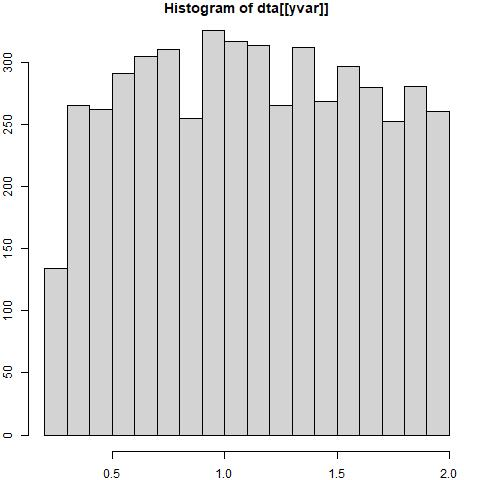
\includegraphics[width=4.5in]{FIGURES/simple_width.jpeg}
\caption{Sample of Histogram generated for the 'Width of Vent' column}
\label{simple_width_hist}
\end{figure}

There is clearly some noise in the data and all the columns are not the same hieght as would be expected in theoretical uniform distribution. However, there really is only one column, the fisrt one, that is significantly out of line with the others. One way of trying to understand why that colum is so much smaller is to go into the {\ct simple\_width.csv} file. In that file the first bar is for the range 0.2 m to 0.3 m but the random generator had a lower bounds of 0.25 m. Doubling the 134 count  puts it right in the middle of the values for the other bars. With that question answered the chart seems to be a reasonable repersentation of a uniform distribution.

In this automatic analysis the number of bins used here is automatically selected using Sturges rule \cite{Sturges_1926} which chooses the number of bins according to the rule: \[k = \lceil \log_2 n \rceil + 1\], where  \[ \lceil \rceil\] represents the ceiling function. While the Sturges rule works well it isn't perfect so be careful of drawing a conclusion to quicly looking at the output of any of the {\ct \&MSTT} tools CData provides. 

\subsubsection{Empirical Probability Density Function}

The post-processor is also capable of generating an empirical probability density function. It does so using the techniques of Kernal Density Estimation \cite{Haste_2009}. To determine the probability density at a point \textit{x} it associates a weight with each point in the data set. The weight is a function of the distance between the point in the data set and \textit{x}. The probability density is then the sum of those weights.

Typically the Gaussian function is used as the Kernal (i.e., the weighting function), although other Kernals are also commonly used. For the Gaussian Kernal (which is used here) the estimated probability density at a point \textit{x} is:

\[f(x) = \frac{1}{Nb}\sum_{j=1}^{N} \phi\left(\frac{x - x_j}{b} \right) \]

where \textit{N} is the number of data points, \[x_j\] is an individual data point, \[\phi\] is the standard normal density function, and \textit{b} is the "bandwidth." The bandwidth determines the width of the window within which the data points contribute significantly to the density estimate. In this implementation, the bandwidth is determined automatically.

\subsubsection{Determining If Enough Runs Have Been Made}

Monte Carlo analysis is fundamentally grounded in The Law of Large Numbers. The Law of Large Numbers states that for a large-enough number of independent samples, the average converges to the expected value. For example, if we want to know what the probability of flashover is in the kitchen for a certain class of fires, the Law of Large Numbers assures us that the percentage of Monte Carlo runs where flashover occurs converges to the probability as the number of runs becomes large.

The problem here is determining how many runs is enough. Put differently, how many runs does it take to guarantee a result that is "close enough" to be usable? Two strategies are used here. The first is graphing the evolution of the mean versus number of runs. The second is to graph the standard deviation of the mean versus the number of runs. The first strategy should show decreasing variation as the number of runs increases and should converge on a point. The second strategy should show the variance decreasing with the number of runs and approaching zero. The determination of whether the estimates are "close enough" is a judgment of the analyst and will depend on how much accuracy is needed.

In this simple example the mean of two outputs {\ct 'Time to Layer Height 1.5 m'} and {\ct 'Maximum Upper Layer Temp'}. Figure \ref{simple_max_temp_mean} shows the convergence of the mean. From this graph it seems clear that the mean has converged and that fewer cases could have been used. 

\begin{figure}[h!]
\centering
\includegraphics[width=4.5in]{FIGURES/simple_max_temp_mean.jpeg}
\caption{Sample of Convergence of mean for maximum upper layer temperature}
\label{simple_max_temp_mean}
\end{figure}

Figure \ref{simple_max_temp_sd} shows the standard deviation, which clearly is tending toward zero. 

\begin{figure}[h!]
\centering
\includegraphics[width=4.5in]{FIGURES/simple_max_temp_sd.jpeg}
\caption{Sample of Convergence of mean for maximum upper layer temperature}
\label{simple_max_temp_sd}
\end{figure}

\subsubsection{Decision Trees}

Sometimes what is of interest is the relationship one variable has to other variables in the output. There are many ways of estimating relationships, but one of the most intuitive is that of Decision Trees. The approach implemented here is closely related to that of Classification and Regression Trees \cite{Haste_2009}. The output of the algorithm is a binary tree. Each node splits the data into two, until the tree arrives at the leaf nodes. For classification trees, each leaf node is associated with the best-fit category. For regression trees, each leaf node is associated with the average of the data that arrives at that node.

Decision trees have the advantage of being very easy to interpret. Their interpretability is one reason for their popularity. Trees have a couple of drawbacks as well. The most noticable is that their predictions are not smooth. In addition, trees can be highly unstable. That is, small changes in the data can produce large changes in the estimated tree. In addition, there are cases the same data can be represented by very different trees.

One of the {\ct \&MSTT} namelists creates a decision tree for maximum layer temperature. Figure \ref{simple_tree_temp} shows the tree. 

\begin{figure}[h!]
\centering
\includegraphics[width=6.5in]{FIGURES/simple_tree_temp.jpeg}
\caption{Sample of Convergence of mean for maximum upper layer temperature}
\label{simple_tree_temp}
\end{figure}

%%%%%%%%
%
% chapter Examples
%
%%%%%%%%%

\chapter{Examples}

%%%%%%%%%
%
% Example 1
%
%%%%%%%%

\section{Example 1: Flashover in a compartment}

The occurrence of flashover within a room is of considerable interest since it is perhaps the ultimate signal of untenable conditions within the room of fire origin and a sign of greatly increased risk to other rooms within the building. Many experimental studies of full-scale fires have been performed that quantify the onset of flashover in terms of measurable physical properties. Several approaches have been taken to estimate the onset of flashover within a room. These methods are typically based on simplified mass and energy balances on a single-compartment fire along with correlations to fire experiments. Walton and Thomas \cite{Walton:2016} provide a review of available methods for calculating temperatures in fires in a single compartment with an open door. Three methods are identified from the works of Babrauskas \cite{Babrauskas:1980}, McCaffrey et al. \cite{McCaffrey:1981uq} and Thomas \cite{Thomas:1981fk}. Additional correlations by Babrauskas \cite{Babrauskas:1980} and H\"ugglund \cite{Hagglund:1980} are available. This example uses the Monte Carlo capabilities in CData to generate a set of data to compare these correlations to a range of CFAST simulations. Figure \ref{flashover_geometry} shows the compartment geometry for the simulations.

\begin{figure}[h!]
\centering
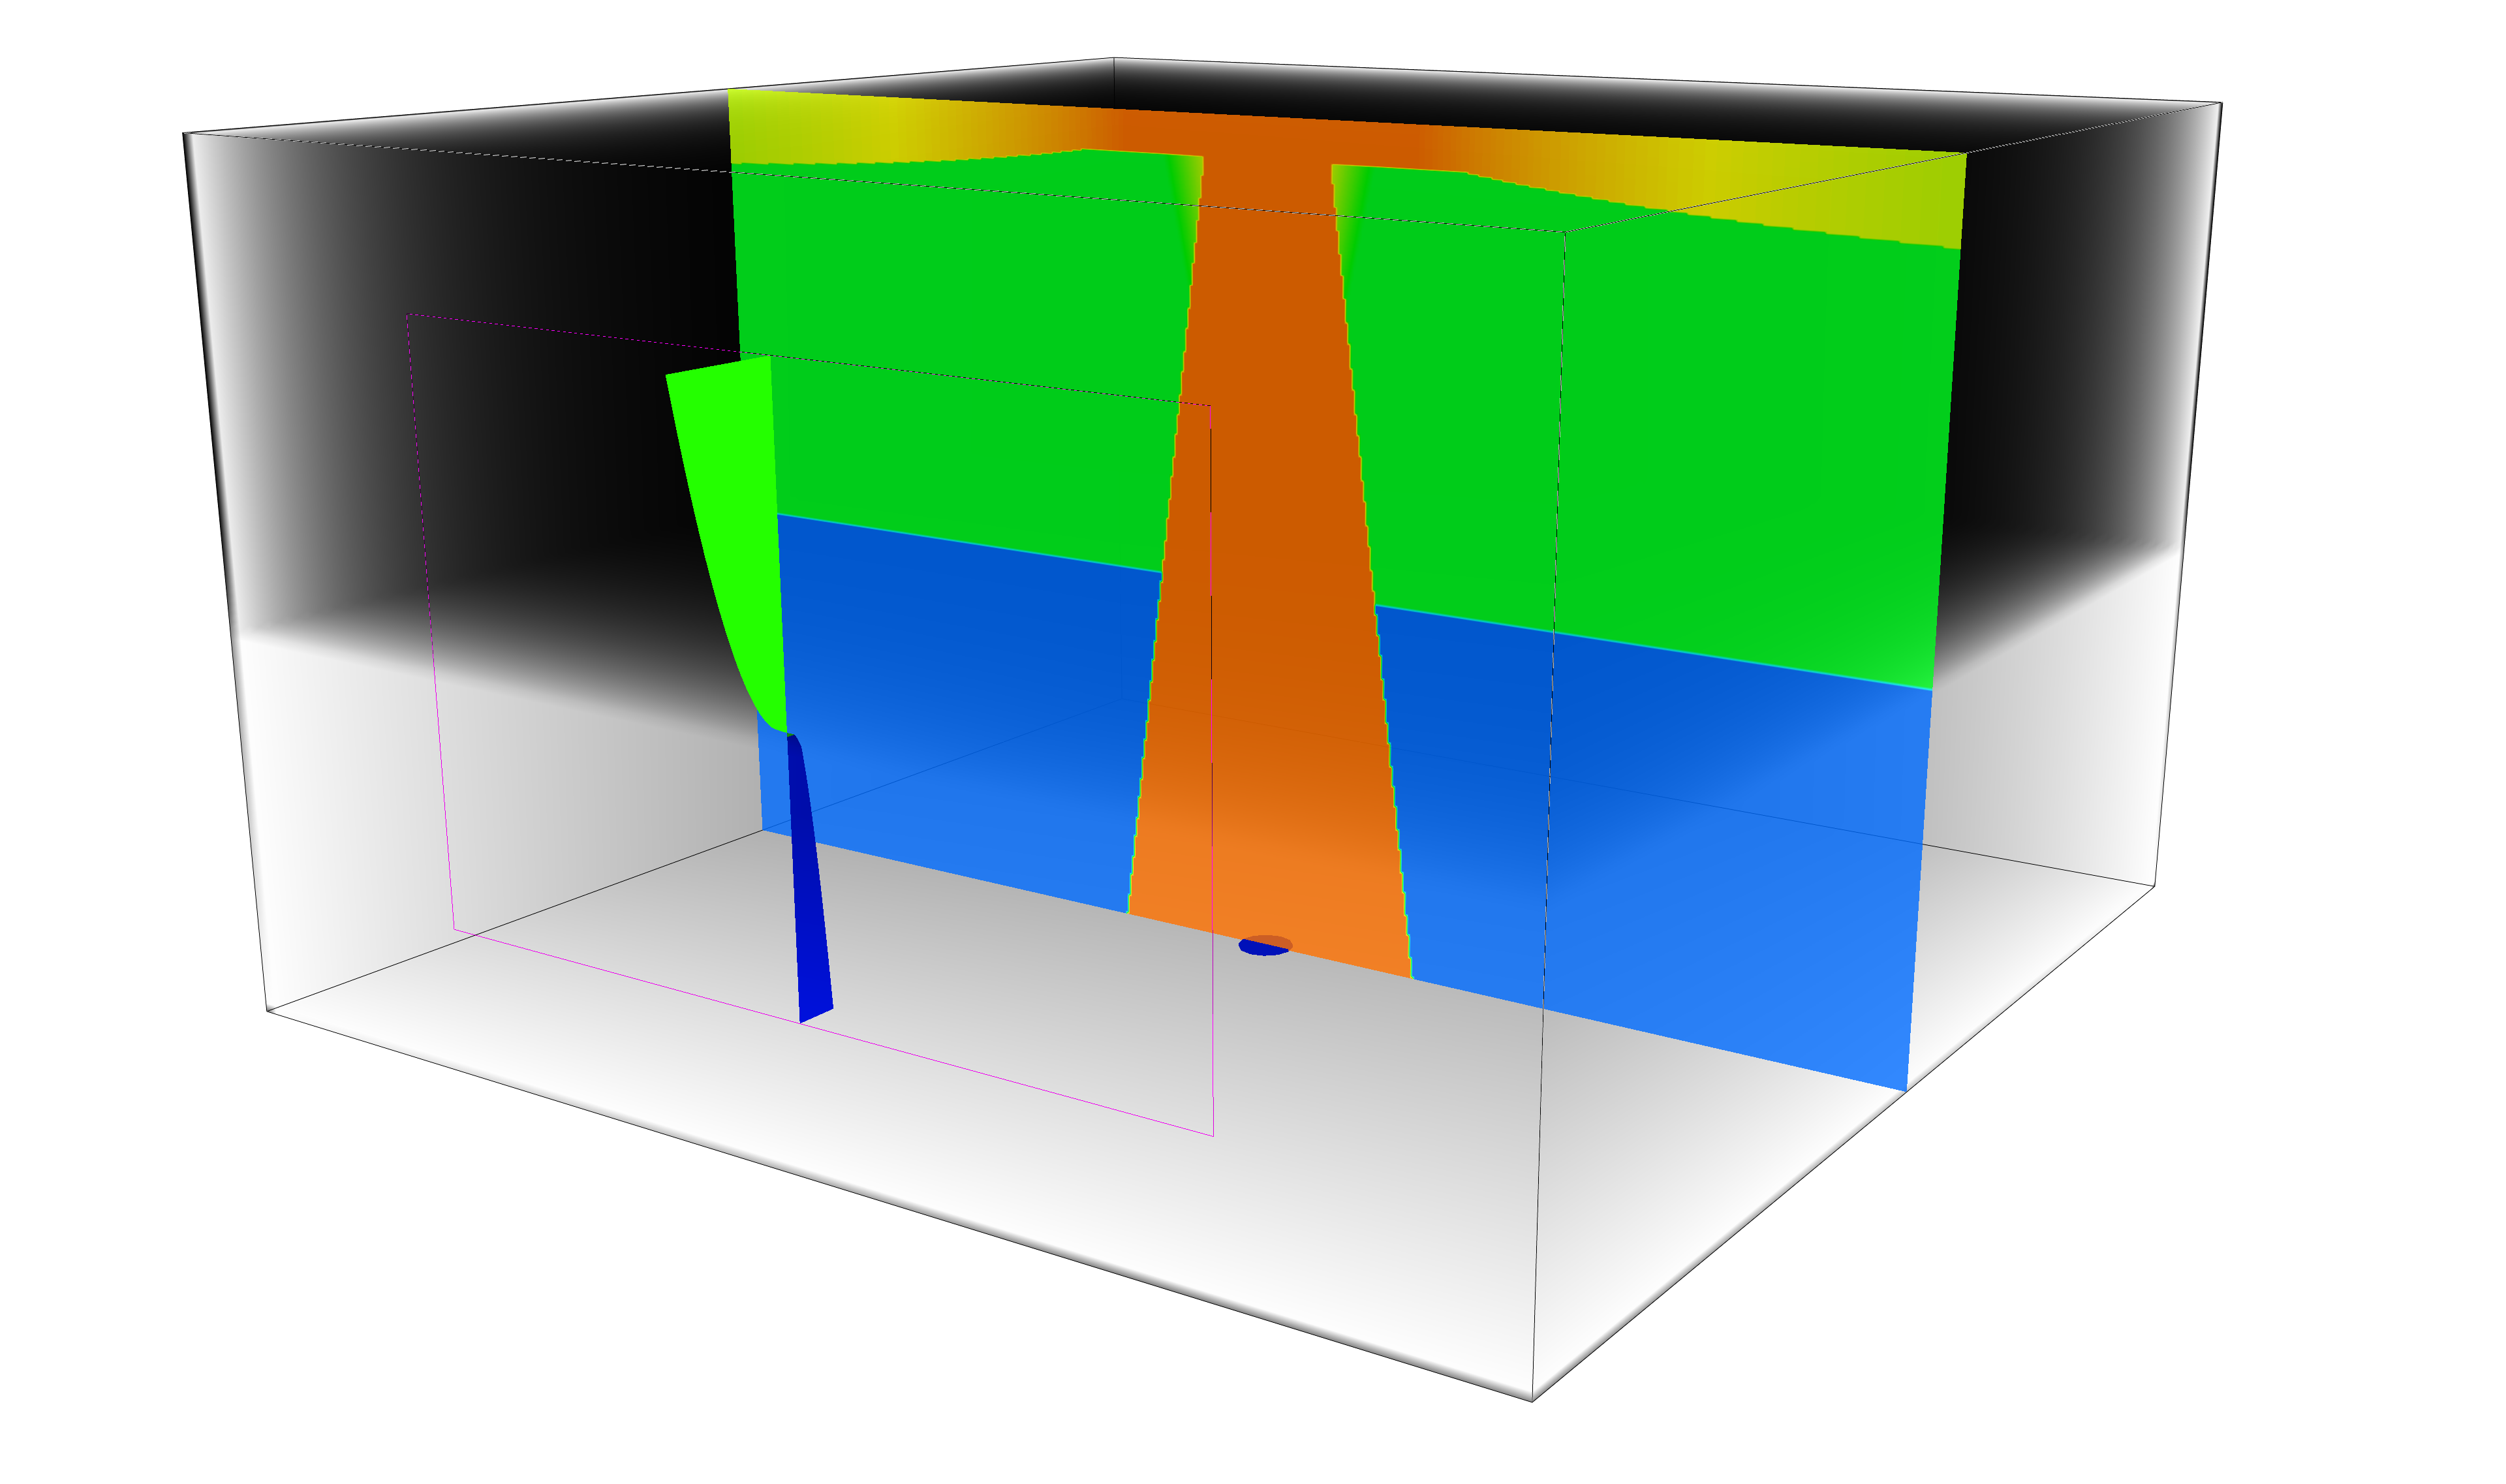
\includegraphics[width=4.5in]{FIGURES/Flashover.png}
\caption{Sample CFAST visualization of a single compartment structure used for example 1.}
\label{flashover_geometry}
\end{figure}

\subsection{CData Inputs}
A single compartment with gypsum ceiling and walls and a concrete floor includes a single vent. For this example, the room dimensions, vent dimensions, and fire growth rate are varied as follows:

\begin{description}
\item[Compartment dimensions:] Compartment sizes varied with a uniform distribution scaling all compartment dimensions from 2 m x 2 m x 2 m to 20 m x 20 m x 20 m.
\item[Vent dimensions:] Vent sizes varied with a uniform distribution scaling vent bottom from 0 m to 1.5 m, a uniform distribution scaling vent top from 1.65 m to 19.85 m limited by compartment height, and a uniform distribution scaling vent width from 0.25 m to 19 m limited by compartment width.
\item[Fire growth rate:] Fire size varied with a uniform distribution ranging from 75 s to 1000 s to 1 the peak heat release rate. Peak heat release rate set to 160 MW to ensure flashover in the largest compartments when there is sufficient oxygen.
\end{description}

For the analysis, we will look at the minimum heat release rate necessary to achieve flashover in the compartment defined by a typically-used metrics of 600 \degc upper layer temperature \cite{Valid:Peacock_Flashover_1} \cite{Valid:Peacock_Flashover_2}.

The compartment size is defined randomly over a range of 2 m to 20 m. The example below varies the room width. Other dimensions are handled in a similar fashion.

\vspace{\baselineskip}
\begin{lstlisting}
&MRND ID = 'Comp 1 Width Generator' DISTRIBUTION_TYPE = 'UNIFORM' VALUE_TYPE = 'REAL'
    MINIMUM = 2.0 MAXIMUM = 20.0/
&MFLD ID = 'Comp 1 Width' FIELD_TYPE = 'VALUE' RAND_ID = 'Comp 1 Width Generator' FIELD = 'Comp 1' 'WIDTH'
    ADD_TO_PARAMETERS = .TRUE. /
\end{lstlisting}

The vent height and width also vary randomly, but must be limited to the compartment height and width. Here, the maximum value for the top of the vent is defined as 0.15 m below the compartment ceiling (specified by the {\ct MAXIMUM\_OFFSET} of -0.15 m, with the negative number indicating an offset relative to the top of the compartment) and the vent width maximum is defined as 1 m less than the vent width (specified by the {\ct MAXIMUM\_OFFSET} of -1.0 m).

\vspace{\baselineskip}
\begin{lstlisting}
&MRND ID = 'Wall Vent Bottom Generator' DISTRIBUTION_TYPE = 'UNIFORM' VALUE_TYPE = 'REAL'
    MINIMUM = 0.0 MAXIMUM = 1.5/
&MFLD ID = 'Wall Vent Bottom' FIELD_TYPE = 'VALUE' RAND_ID = 'Wall Vent Bottom Generator' FIELD = 'Wall Vent' 'BOTTOM'
    ADD_TO_PARAMETERS = .TRUE. /

&MRND ID = 'Wall Vent Top Generator' DISTRIBUTION_TYPE = 'UNIFORM' VALUE_TYPE = 'REAL'
    MINIMUM = 1.65 MAXIMUM_FIELD = 'Comp 1 Height' MAXIMUM_OFFSET = -0.15/
&MFLD ID = 'Wall Vent Top' FIELD_TYPE = 'VALUE' RAND_ID = 'Wall Vent Top Generator' FIELD = 'Wall Vent' 'TOP'
    ADD_TO_PARAMETERS = .TRUE. /

&MRND ID = 'Wall Vent Width Generator' DISTRIBUTION_TYPE = 'UNIFORM' VALUE_TYPE = 'REAL'
    MINIMUM = 0.25 MAXIMUM_FIELD = 'Comp 1 Width' MAXIMUM_OFFSET = -1.0/
&MFLD ID = 'Wall Vent Width' FIELD_TYPE = 'VALUE' RAND_ID = 'Wall Vent Width Generator' FIELD = 'Wall Vent' 'WIDTH'
    ADD_TO_PARAMETERS = .TRUE. /
\end{lstlisting}

The fire specification is naturally the most complex. For this example, we use a t-squared growth rate fire that grows to a peak value in a time period from 75 s to 1000 s, followed by a 10 s plateau and 10 s decay back to 0~kW. Since both the plateau and decay are set to 10 s, the same generator input can be used for both time points.
\vspace{\baselineskip}
\begin{lstlisting}
&MRND ID = 'End of Time Growth Generator', DISTRIBUTION_TYPE = 'UNIFORM' VALUE_TYPE = 'REAL'
    MINIMUM = 75 MAXIMUM = 1000 /
&MRND ID = 'Plateau End Time' DISTRIBUTION_TYPE = 'CONSTANT' VALUE_TYPE = 'REAL' REAL_CONSTANT_VALUE = 10 /
&MRND ID = 'Fire End Time' DISTRIBUTION_TYPE = 'CONSTANT' VALUE_TYPE = 'REAL' REAL_CONSTANT_VALUE = 10 /

&MRND ID = 'Peak HRR Generator', DISTRIBUTION_TYPE = 'UNIFORM' VALUE_TYPE = 'REAL' MINIMUM = 1500000 MAXIMUM = 160000000/
&MRND ID = 'End of Fire HRR' DISTRIBUTION_TYPE = 'CONSTANT' VALUE_TYPE = 'REAL' REAL_CONSTANT_VALUE = 0 /

&MFIR ID = 'Fire_generator' FIRE_ID = 'New Fire 1' FIRE_TIME_GENERATORS = 'End of Time Growth Generator'
    'Plateau End Time' 'Fire End Time' FIRE_HRR_GENERATORS = 'Peak HRR Generator' 'Peak HRR Generator'
    'End of Fire HRR' NUMBER_OF_GROWTH_POINTS = 20 GROWTH_EXPONENT = 2 /
\end{lstlisting}

\subsection{Analysis}

Flashover is a term describing the transition of a relatively localized interior fire to one engulfing the entire compartment. It is of interest to the fire service because of the danger to fire fighters and to building designers because of life safety and the attendant impact on occupants. Several papers have looked at the capability of CFAST to predict the conditions under which flashover can occur \cite{Valid:Chow_Flashover, Valid:Luo_Flashover, Valid:Collier, Valid:White}. In addition, a comparison of CFAST with a number of simple correlations was used by Peacock and Babrauskas \cite{Valid:Peacock_Flashover_1,Valid:Peacock_Flashover_2} to simulate a range of geometries and fire conditions to predict the development of the fire up to the point of flashover. The important test of  these prediction methods is in the comparison of the predictions with actual fire observations. Figure \ref{figValidFlashover} (reference \cite{Valid:Peacock_Flashover_2}) presents estimates of the energy required to achieve flashover for a range of room and vent sizes from the CFAST runs above. This figure is an extension of the earlier work of Babrauskas  \cite{Valid:Babrauskas_Flashover} and includes additional experimental measurements from a variety of sources, most notably the work of Deal and Beyler \cite{Valid:DealandBeyler}. For a number of the experimental observations, values are included that were not explicitly identified as being a minimum value at flashover.

\begin{figure}
\begin{center}
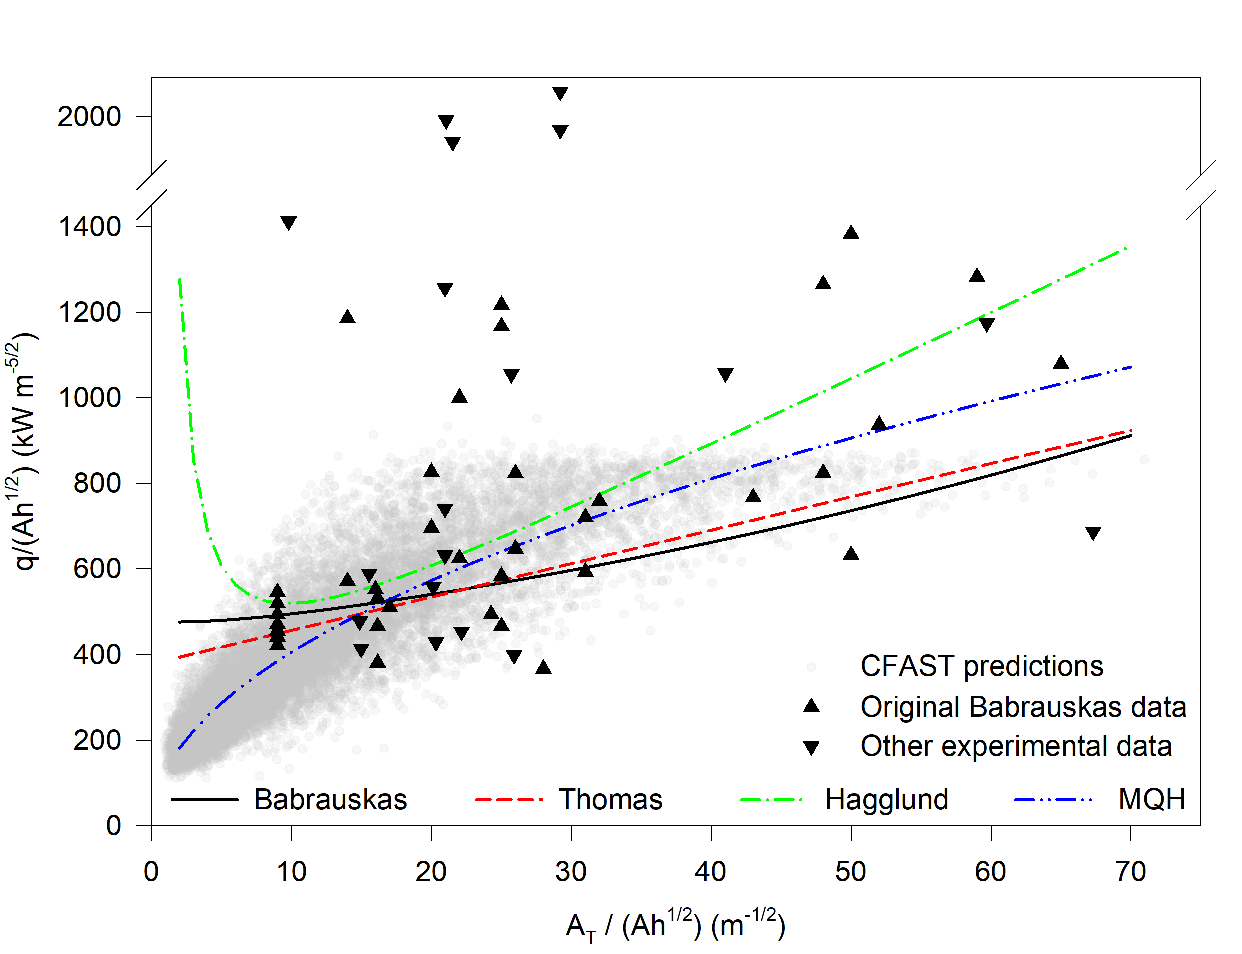
\includegraphics[width=6.0000in]{../Validation_Guide/FIGURES/flashover.pdf}\\
\end{center}
\caption{Comparison of correlations, CFAST predictions, and experimental data for the prediction of flashover in a compartment fire.}
 \label{figValidFlashover}
\end{figure}

%%%%%%%%%
%
%  Example 2
%
%%%%%%%%%%

\section{Example 2: Impact of smoke detector interconnection}

Battery-powered smoke alarms with wireless interconnect signal transmission allow for retrofitting of homes with interconnected smoke alarms up to the current code-required installation locations without hardwiring. However, wireless communication draws additional current beyond basic smoke alarm operation and will affect battery life. To receive an interconnect signal, wireless smoke alarms must periodically power up the transceiver and listen for a transmitted signal from another alarm that initially responds to smoke. Naturally a question arises: what is an acceptable maximum delay time for wireless interconnected smoke alarms given the desire to extend battery life?

\subsection{CData Inputs}
In this simplified example based on earlier work \cite{Cleary_2019}, we look at the impact of a periodic activation of wireless communications in detectors. We will use a fixed single-story residential structure for the simulations, varying the fire placement and size, the opening/closing of doors within the structure, and the properties of the smoke detectors placed in each compartment. Figure \ref{detector_geometry} shows the compartment geometry for the simulations.

\begin{figure}[h!]
\centering
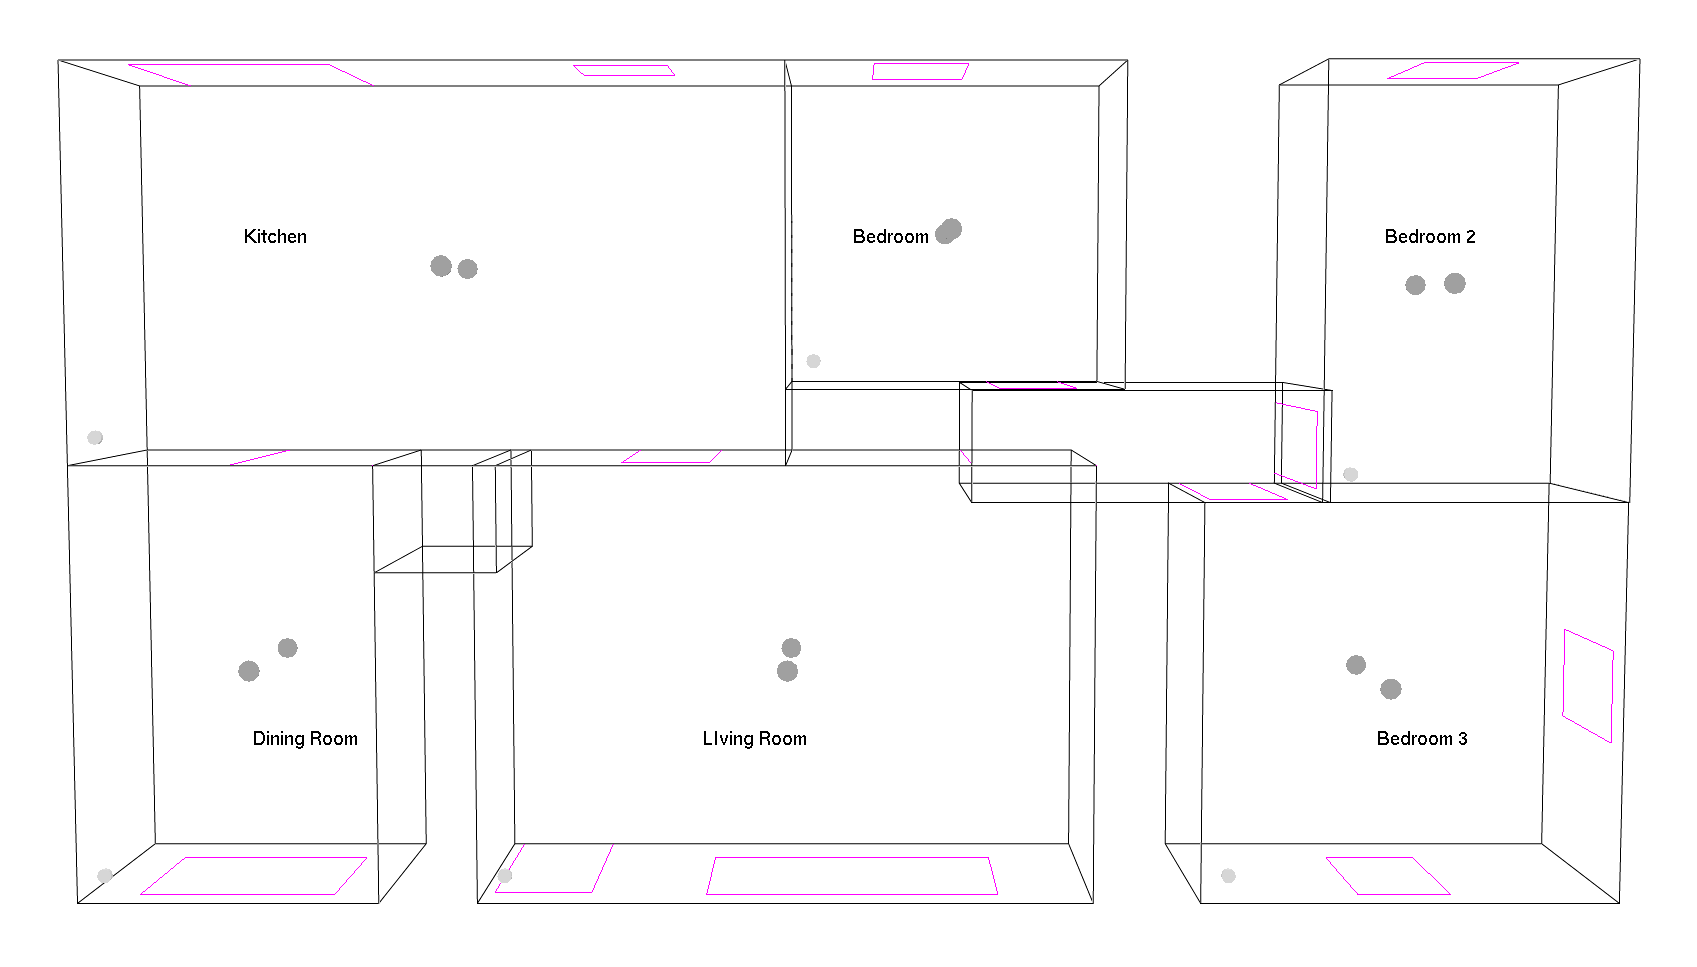
\includegraphics[width=6.5in]{FIGURES/Detectors.png}
\caption{Sample CFAST visualization of a single story residential structure used for example 2.}
\label{detector_geometry}
\end{figure}

For this example, the fire location, fire growth, fire peak heat release rate, vent opening/closing for all interior vents, and smoke detector sensitivity will be varied as follows:

\begin{description}
\item[Fire location:] Fire is placed in a fixed location in a randomly chosen compartment in the structure and is equally split between flaming and smoldering fires.
\item[Initial fire growth rate:] Flaming fires grow from zero to 23~kW $\pm$ 7~kW in 207~s $\pm$ 46~s using normal distributions, followed by a t$^2$ growth to 1054~kW in 222~s $\pm$ 47~s again using a normal distribution. Smoldering fires grow from zero to 11~ kW $\pm$ 3~kW in 6863~s $\pm$ 1812~s using normal distributions, followed by a t$^2$ growth to 1054~kW in 189~s $\pm$ 48~s again using a normal distribution.
\item[Interior doors:] Doors between all interior compartments are each randomly set to be initially fully open or with a 2.5~cm undercut the full width of the door. These openings remain unchanged throughout a simulation.
\item[Smoke detectors:] Smoke detectors follow a statistical smoke alarm activation model developed for upholstered furniture containing polyurethane foam \cite{Cleary:2017}. For this simple example,we use only one detector who activation varies with a log-normal distribution with a geometric mean of 9.5 \%/m $\pm$ 4.2 \%/m (3.0~\%/ft $\pm$ 1.3 \%/ft) for flaming fires and 15.5 \%/m $\pm$ 4.2 \%/m (5.0~\%/ft $\pm$ 1.3 \%/ft) for smoldering fires.
\end{description}

In the analysis, we will look at the impact of delays in triggering of secondary, interconnected smoke detectors on the overall tenability for a range of fires.


\hypertarget{data}{%
\subsection{Data}\label{data}}

The information on doors is not really in a usable form, so for this analysis the door information is recoded into a door state for each door. The state can be one of ``closed'' ``one-fourth'', ``one-half'', ``three-fourth'', and ``open.'' The recoding for doors is what is used throughout this analysis.

\hypertarget{number-of-cases}{%
\subsection{Number of Cases}\label{number-of-cases}}

As a first step, we do a preliminary check to see if we have enough cases, Figs. \ref{Ex_3-convergence_of_mean} and \ref{Ex_3-standard_error}.

\begin{figure}[h!]
\centering
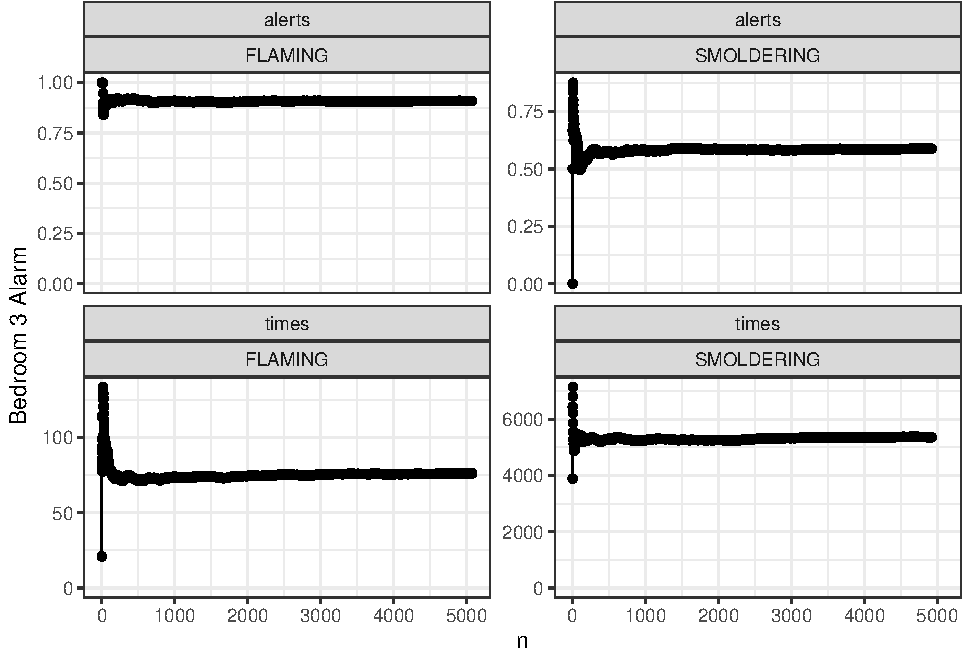
\includegraphics[width=4.5in]{FIGURES/converg-1.pdf}
\caption{Mean percent activation and time to activation for the bedroom 1 alarm as a function of the number of cases.}
\label{Ex_3-convergence_of_mean}
\end{figure}
\begin{figure}[h!]
\centering
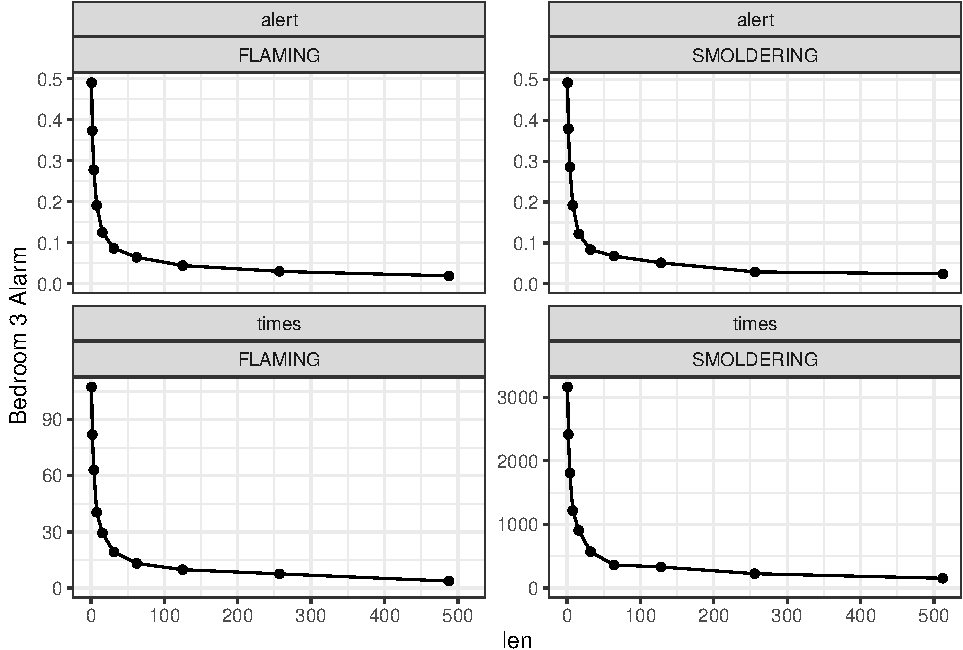
\includegraphics[width=4.5in]{FIGURES/converg-2.pdf}
\caption{Standard deviation of percent activation and time to activation for the bedroom 1 alarm as a function of the number of cases.}
\label{Ex_3-standard_error}
\end{figure}

To be meaningful we have to look at one of the output columns; here we look at the Bedroom 1 Alarm data. Looking at the data it becomes very quickly apparent that the results for Flaming type fires and Smoldering type fires are very different. Also, nearly half the cases have no activation within the simulation time. So the evaluation of convergence is evaluated separately for flaming type fires and smoldering type fires. Then the time to activation for cases where activation occurs is evaluated separately from the percent of cases where activation occurs. If any of these do not converge, then we do not have enough cases.

The preliminary results suggest that we have enough cases. The averages all appear to have converged, and the standard errors are small.

\hypertarget{analysis}{%
\subsection{Analysis}\label{analysis}}

The question explored here is the benefit gained by connecting alarms. The effect of interconnecting alarms is to reduce the amount of time before people in the house are notified of a fire even though they may be far away from the location of the fire. In this example, there are fires in the dining room, kitchen, or living room, and we will assume that people are in the bedrooms. Further assume the people in the bedrooms will not hear an alarm unless it is the one in the bedroom. So the effect of interconnecting alarms is to notify people to a fire when the alarm in one of the front rooms goes off rather than waiting until one of the bedroom alarms sounds.

Assume for this example that there is one alarm in the Living Room and one alarm in Bedroom 1 (which will proxy for all the bedroom alarms). This example, then, examines the difference in activation times between the Living Room Alarm and the Bedroom 1 Alarm.

Exploratory analysis of the data is an important part of any analysis. Here, initial exploration indicated that in a substantial number of cases one or more of the alarms never activated.

\noindent
\begin{table}[ht]
\begin{center}
\caption[Number of cases by alarm activation status.]{Number of cases by alarm activation status.}
\label{tbl:Ex_3-1}
\begingroup
\renewcommand{\arraystretch}{1.2}
\begin{tabular}{@{\extracolsep{\fill}}|l|l|l|l|l|}
\hline
\parbox{1.5in}{ }    & \parbox{1in}{\bf Bedroom 1}  & \parbox{1in}{\bf No} & \parbox{1in}{\bf Yes}  & \parbox{1in}{\bf NA}  \\ \hline
Living Room &  &   &   &   \\
No &  & 738 & 0 & 0 \\
Yes &  & 3309 & 5929 & 0 \\
NA &  & 0 & 0 & 24 \\ \hline
\end{tabular}
\endgroup
\end{center}
\end{table}

Table \ref{tbl:Ex_3-1} displays the number of cases where each of the alarms activated. Cases marked NA, are cases where the model itself did not converge. That was a very small number of cases for this example.

For more than half the cases, both alarms activated. For most of the remaining cases the Living Room alarm activated but the Bedroom alarm did not. For less than 10~\% of the cases neither alarm activated. There were no cases where the bedroom alarm activated but the Living Room alarm did not.

To better understand the cases where the bedroom alarm fails to sound, a classification tree was generated on whether the bedroom alarm sounded (Fig \ref{Ex_3-classification_tree}). It is unusual for a tree to produce results as stark as this one. What becomes clear on looking at the tree is that the state of the intervening doors determines whether the bedroom alarm sounds. If the fire is isolated from the bedroom by closed doors then the alarm will not sound. Otherwise it will.

Interconnected alarms do not monitor continuously. Rather they check periodically to see if some other alarm has sounded. For this example, we will assume they check every 60 seconds. The effect is that there is a random delay, with the delay drawn from a uniform random distribution of between 0 s and 60 s. A Kernal Density estimate of the distribution of time savings is shown in Fig \ref{Ex_3-distributions}, with fire type on separate charts. Any negative ``time delay'' means that the bedroom alarm sounds on its own before it gets notification from the Living Room alarm.

\begin{figure}[h!]
\centering
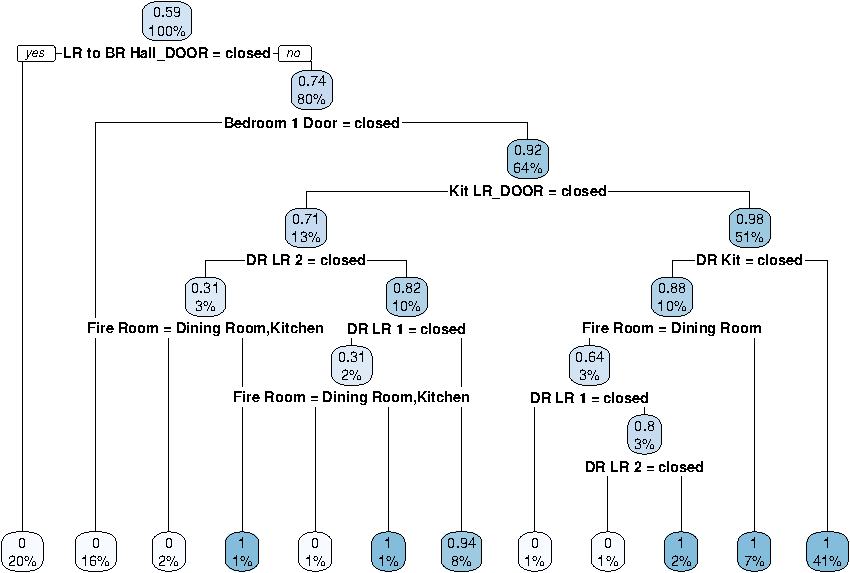
\includegraphics[width=4.5in]{FIGURES/cart-1.pdf}
\caption{Classification tree separating cases where the bedroom alarm sounded from those where it did not.}
\label{Ex_3-classification_tree}
\end{figure}
\begin{figure}[h!]
\centering
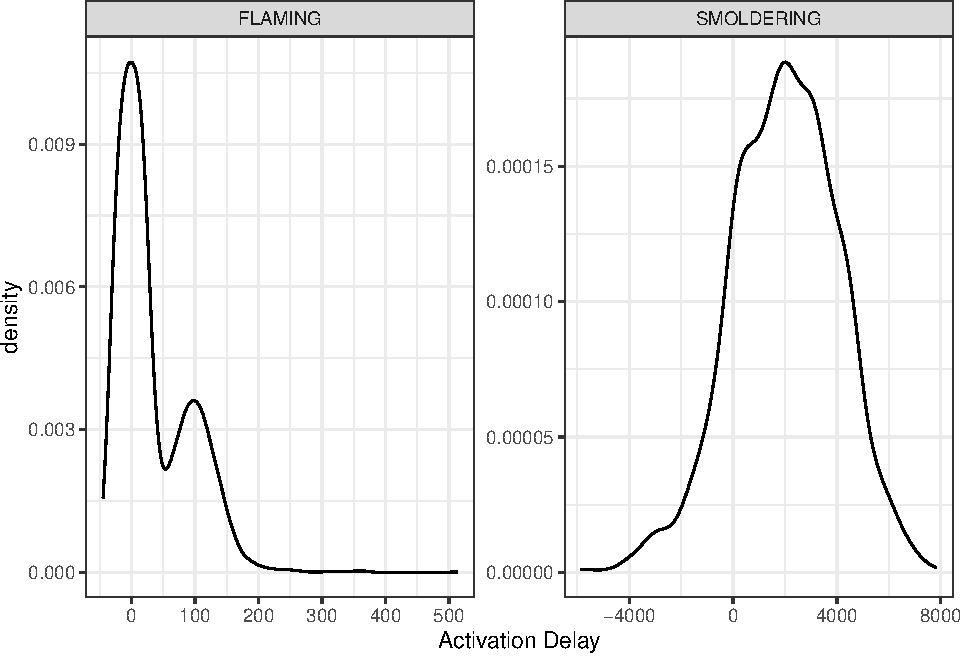
\includegraphics[width=4.5in]{FIGURES/kde-1.pdf}
\caption{Kernel Density estimate of the time savings for interconnected alarms by fire type.}
\label{Ex_3-distributions}
\end{figure}

With 10~000 data points we can empirically estimate the average time savings that interconnected alarms would provide, as well as median time savings and various quantiles. We are interested in the quantiles because adverse outcomes, like death or injury, are tail events. So we also look at the tails of the distribution. Here the ``1~\% Quantile'' means that 1~\% of alarms saved more time than this (see Table \ref{tbl:Ex_3-2}.

\noindent
\begin{table}[ht]
\begin{center}
\caption[Quantiles of delay time for bedroom alarm activation]{Quantiles of delay time for bedroom alarm activation}
\label{tbl:Ex_3-2}
\begingroup
\renewcommand{\arraystretch}{1.2}
\begin{tabular}{@{\extracolsep{\fill}}|l|l|l|}
\hline
\parbox{1.5in}{\bf Result}    & \parbox{0.75in}{\bf Flaming}  & \parbox{1in}{\bf Smoldering}  \\ \hline
Mean & 101.7 & 1821.8 \\
Median & 96.0 & 1597.7 \\
25 \% Quantile & 136.3 & 2936.7 \\
10 \% Quantile & 176.4 & 4139.8 \\
5 \% Quantile & 199.5 & 4792.5 \\
1 \% Quantile & 238.3 & 6109.8 \\ \hline
\end{tabular}
\endgroup
\end{center}
\end{table}

This looks only at cases where the Bedroom 1 alarm sounded. If this were a serious attempt to identify the effect of interconnected alarms then the percent of non-activations would need to be taken into account. If non-activations were included all the quantiles larger than the median would fall into the non-activation range.

\hypertarget{number-of-cases---revisited}{%
\subsection{Number of Cases - Revisited}\label{number-of-cases---revisited}}

The preliminary analysis above suggested that we appeared to have enough cases. However, the values of interest here are complex manipulations of the data. Even though the average of the Bedroom activation time has converged, it is possible that the results of interest to us have not. To finally determine if we have enough cases we look at how the outcomes we analyze change with the number of cases (Fig \ref{Ex_3-quintiles}).

\begin{figure}[h!]
\centering
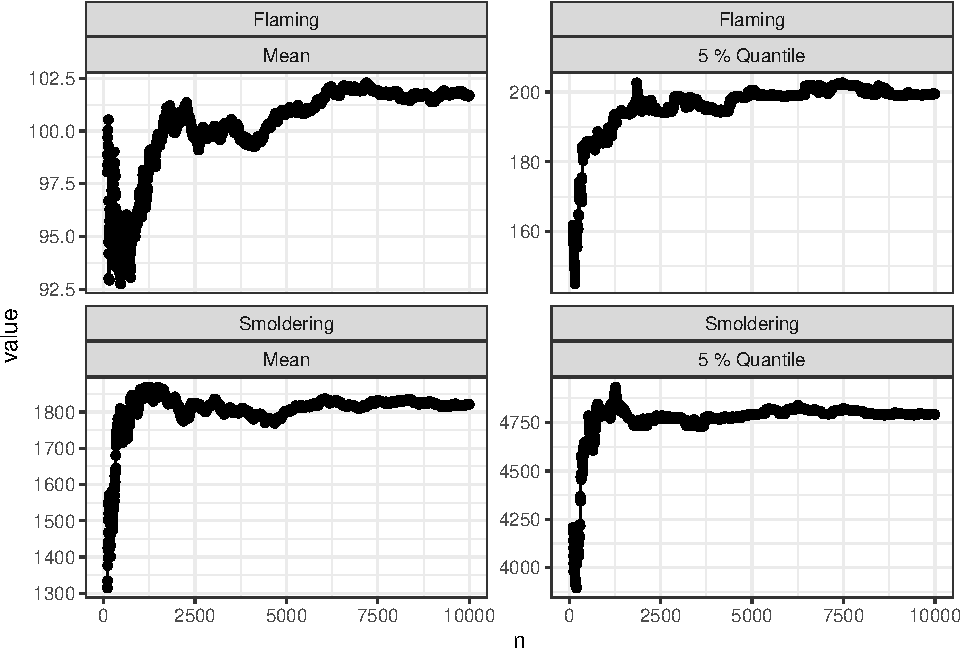
\includegraphics[width=4.5in]{FIGURES/cvg_plot-1.pdf}
\caption{Quantiles of the time savings as a function of the number of cases.}
\label{Ex_3-quintiles}
\end{figure}

While the preliminary look settled down within a couple of thousand cases, these results take longer. In particular the extreme quantiles take somewhat longer to settle down. In particular, the 5 \% quantile value doesn't really settle down until we have 7500 cases or so. However, looking at the results it looks like our results have settled down sufficiently by the 10~000 cases we actually use to have reasonable confidence in our results.

\hypertarget{discussion}{%
\subsection{Discussion}\label{discussion}}

For a study like this it is really important to get the distribution of fire parameters correct. For example, if the proportion of fires starting in the Kitchen were low compared to the real world then all of the time-delay values would be underestimated. If the likelihood of closed doors were overestimated, then there would be far fewer cases of alarm failure for the bedroom alarms, and the benefit of interconnection would be lower.

%%%%%%%%%%
%
% Example 3
%
%%%%%%%%%%

\section{Example 3: Model Sensitivity}

In this example, we look at a simple fire model sensitivity analysis, which ASTM E 1355 defines as a study of how changes in model parameters affect the results \cite{CFAST:ASTM:E1355}. In other words, sensitivity refers to the rate of change of the model output with respect to input variations. The standard also indicates that model predictions may be sensitive to (1) uncertainties in input data, (2) the level of rigor employed in modeling the relevant physics and chemistry, and (3) the accuracy of numerical treatments. Thus, the purpose of a sensitivity analysis is to assess the extent to which uncertainty in the model inputs is manifested as uncertainty in the model results of interest. For this simple example, we will use a single office building and look at the impact of changing important model inputs by $\pm 10$ \%. Figure \ref{sensitivity_geometry} shows the compartment geometry for the simulations.

\begin{figure}[h!]
\centering
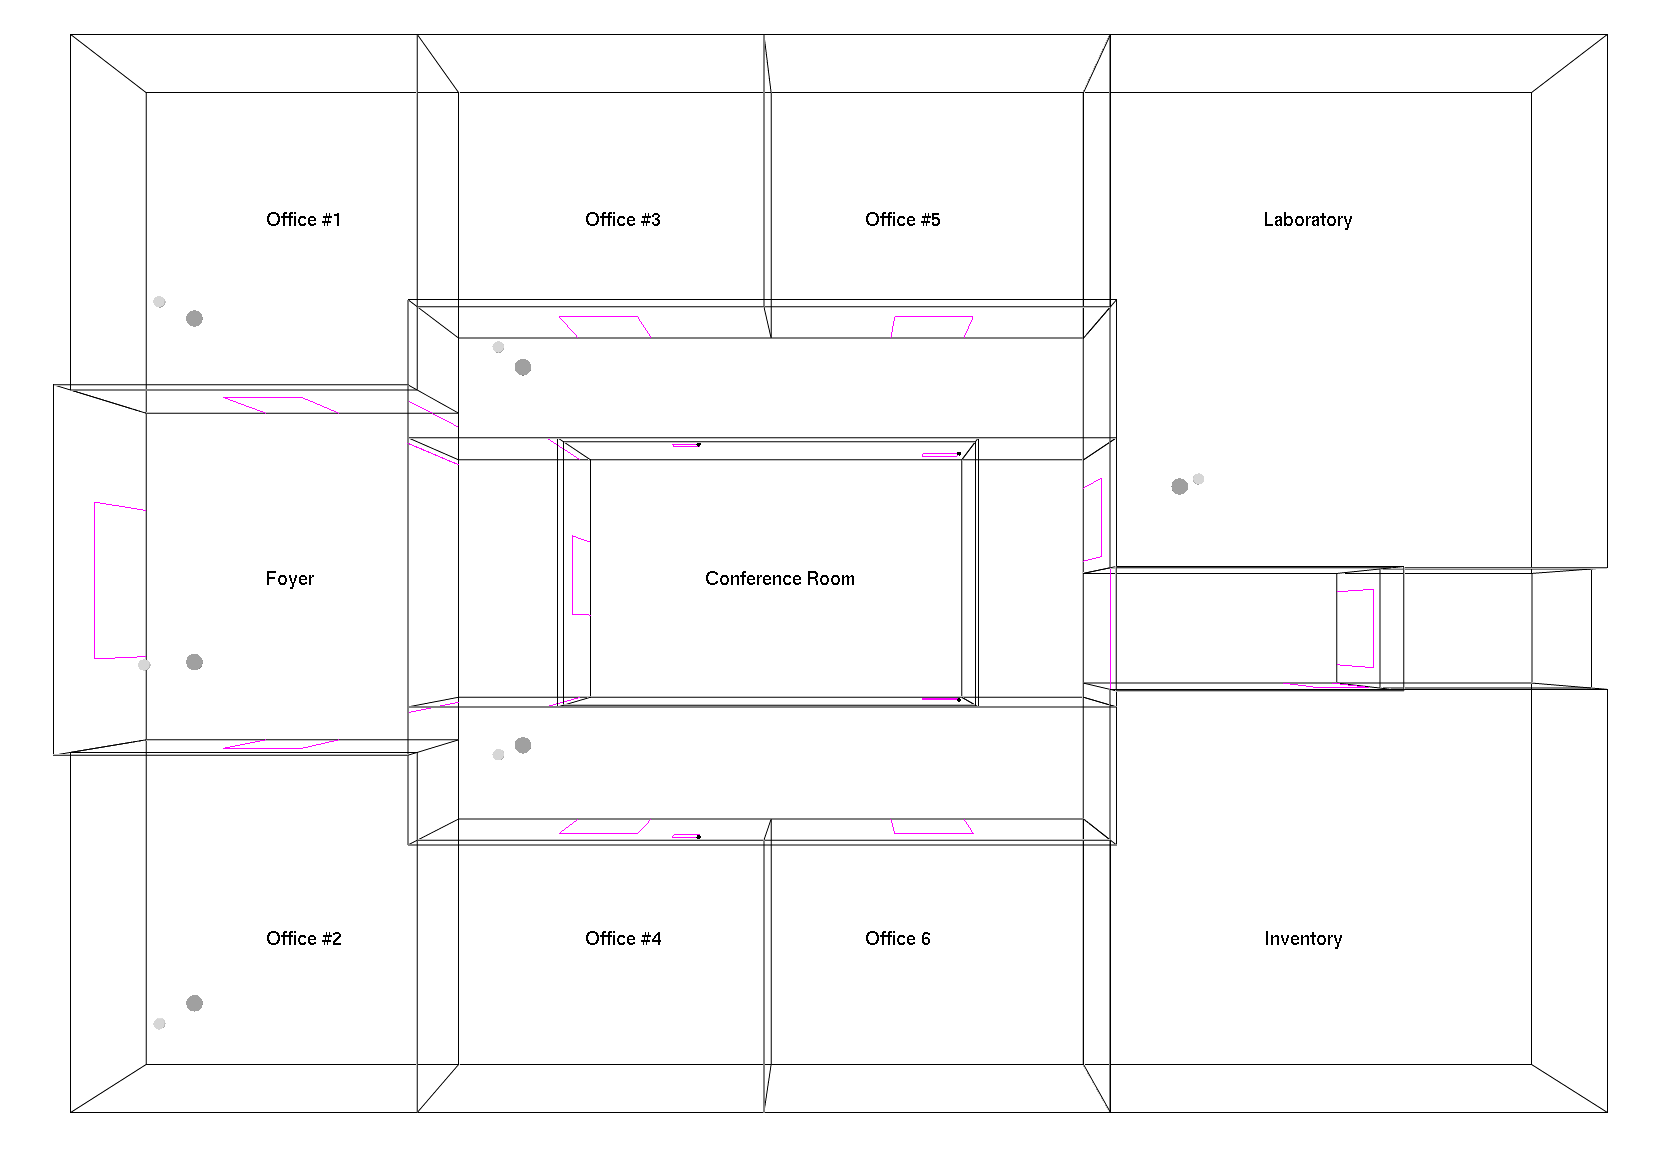
\includegraphics[width=6.5in]{FIGURES/Sensitivity.png}
\caption{Sample CFAST visualization of a single story commercial structure used for example 3.}
\label{sensitivity_geometry}
\end{figure}

A sensitivity analysis involves defining a base case scenario, and varying selected input parameters. The resultant variations in the model output are then measured with respect to the base case scenario, in order to consider the extent to which uncertainty in model inputs influences model output. Therefore, a sensitivity analysis of CFAST should account for variations in the extensive number of input parameters that describe the building geometry, compartment connections, construction materials, and description of one or more fires.

\subsection{CData Inputs}
For this example, we will independently vary the following inputs by $\pm$~10~\%, recognizing that these are not an exhaustive list of input variables, but which should represent the major model inputs to a simulation:

\begin{description}
\item[Compartment geometry:] Compartment size will be scaled to $\pm$ 10~\% of base size in all dimensions.
\item[Compartment materials:] Thermal properties for all materials will be varied by $\pm$ 10~\% of base values for thermal conductivity, density, and specific heat. Thickness will be  varied by $\pm$ 10~\% of base values.
\item[Compartment doors:] The size of compartment doors, both interior and exterior, will be  varied by $\pm$ 10~\% of base values for height and width. All interior vents will be open for this example.
\item[Mechanical ventilation:] For mechanical ventilation, the height of each vent, area of each vent, and fan flowrate will each be varied by $\pm$ 10~\% of base values.
\item[Fire:] Fire is in one of the rooms. Peak heat release rate of the fire and time of the peak will be varied by $\pm$ 10~\% of base value. Yields of carbon monoxide and soot will each be varied by $\pm$ 10~\% of base value. Position of the fire is varied by $\pm$ 10~\% of base values in width and depth, and height.
\item[Detectors:] Sensitivity of heat detectors will be varied by $\pm$ 10~\% of base values for activation temperature and RTI. Smoke detector activation obscuration will be varied by $\pm$ 10~\% of base values.
\end{description}

In the analysis, we will look at typically-used outputs to determine those which are more sensitive (a 10 ~\% change in an input value leads to more than a 10~\% change in an output) and less sensitive (a 10 ~\% change in an input value leads to less than a 10~\% change in an output) to a change in selected model inputs to identify the relative importance of selected model inputs to the results of a simulation.

Since this case is looking at varying almost everything that can be varied it is the largest file of the three examples. It is possible to actually vary the generators over the range that the variable can take but that means a lot of data entry that could easilly lead to errors that would be difficult to find. One FIELD\_TYPE is the SCALING type. Using this greatly increases the speed of creating the input file.

As part of the inputs one of the things to keep in mind is that the foyer and halls should be the same hieght becasue they are all essentially the same space even though in CFAST they are modeled with a number of compartments and connections. The result is that there is a single random generator that is used by all the rooms and connections making up the halls of the structure as can be seen in the following input snippet.


\vspace{\baselineskip}
\begin{lstlisting}
&MRND ID = 'Scaling height', FYI = 'Scaling for everything that has the same max height', DISTRIBUTION_TYPE = 'UNIFORM',
    VALUE_TYPE = 'REAL', MINIMUM = 0.9 MAXIMUM = 1.1 /
&MFLD ID = 'Foryer height' FIELD_TYPE = 'SCALING' FIELD = 'Foyer'  'HEIGHT'
    RAND_ID = 'Scaling height' ADD_TO_PARAMETERS = .TRUE. PARAMETER_HEADER = 'Foyer_and_Halls_height' /
&MFLD ID = 'Even Hallway height' FIELD_TYPE = 'SCALING' FIELD = 'Even Hallway'  'HEIGHT' RAND_ID = 'Scaling height' /
&MFLD ID = 'Odd Hallway height' FIELD_TYPE = 'SCALING' FIELD = 'Odd Hallway'  'HEIGHT' RAND_ID = 'Scaling height' /
&MFLD ID = 'Front Hall height' FIELD_TYPE = 'SCALING' FIELD = 'Front Hall'  'HEIGHT' RAND_ID = 'Scaling height' /
&MFLD ID = 'Back Hall height' FIELD_TYPE = 'SCALING' FIELD = 'Back Hall'  'HEIGHT' RAND_ID = 'Scaling height' /
&MFLD ID = 'Bathroom Hallway height' FIELD_TYPE = 'SCALING' FIELD = 'Bathroom Hall'  'HEIGHT' RAND_ID = 'Scaling height' /
&MFLD ID = 'Foyer2FrontHall height' FIELD_TYPE = 'SCALING' FIELD = 'Foyer2FrontHall'  'TOP' RAND_ID = 'Scaling height' /
&MFLD ID = 'Foyer2EvenHall height' FIELD_TYPE = 'SCALING' FIELD = 'Foyer2EvenHall'  'TOP' RAND_ID = 'Scaling height' /
&MFLD ID = 'Foyer2OddHall height' FIELD_TYPE = 'SCALING' FIELD = 'Foyer2OddHall'  'TOP' RAND_ID = 'Scaling height' /
&MFLD ID = 'FrontHall2EvenHall height' FIELD_TYPE = 'SCALING' FIELD = 'FrontHall2EvenHall'  'TOP' RAND_ID = 'Scaling height' /
&MFLD ID = 'FrontHall2OddHall height' FIELD_TYPE = 'SCALING' FIELD = 'FrontHall2OddHall'  'TOP' RAND_ID = 'Scaling height' /
&MFLD ID = 'BackHall2EvenHall height' FIELD_TYPE = 'SCALING' FIELD = 'BackHall2EvenHall'  'TOP' RAND_ID = 'Scaling height' /
&MFLD ID = 'BackHall2OddHall height' FIELD_TYPE = 'SCALING' FIELD = 'BackHall2OddHall'  'TOP' RAND_ID = 'Scaling height' /
\end{lstlisting}

After all the fields that are to be varied are set up there is also the fire to vary. Instead of varying the fire we will scale the HRR and time with single indepent scaling factors. This requires only two random generators and is implemented as follows.

\vspace{\baselineskip}
\begin{lstlisting}
&MRND ID = 'Scaling HRR', FYI = 'Just making sure it works', DISTRIBUTION_TYPE = 'UNIFORM',
    VALUE_TYPE = 'REAL', MINIMUM = 0.9 MAXIMUM = 1.1 /
&MRND ID = 'Scaling Time', FYI = 'Just making sure it works', DISTRIBUTION_TYPE = 'UNIFORM',
    VALUE_TYPE = 'REAL', MINIMUM = 0.9 MAXIMUM = 1.1 /
&MFIR ID ='Scale fire' FIRE_ID = 'Fire' BASE_FIRE_ID = 'Back Fire' SCALING_FIRE_HRR_RANDOM_GENERATOR_ID = 'Scaling HRR'
    SCALING_FIRE_TIME_RANDOM_GENERATOR_ID = 'Scaling Time' ADD_HRR_SCALE_TO_PARAMETERS = .TRUE. ADD_TIME_SCALE_TO_PARAMETERS = .TRUE. /
\end{lstlisting}

The other advantage, besides ease of implementation, is that it eliminates the possibility of variatiion of individual time points reducing the impact of the variability. For example if one point has the HRR increaseing by some amount but the next HHR value decreses it won't completely average out but it could reduce the impact on the overall scenareo.

\hypertarget{approach}{%
\subsection{Approach}\label{approach}}

For this example it is assumed that the output variables of interest are `Foyer Max Heat FED' and `Foyer Heat FED'. Notionally, we might say that we are interested in the amount of time people have to escape (representedby the time during which they foyer--through which they must evacuate--remains viable) and the worst temperature they might have to face in the Foyer during that evacuation.

Sensitivity analysis is interested in the sensitivity the output has to each input. This is typically expressed in terms of the percent variation in output produced by a one percent variation in each input. As it turns out, simple linear regression of the \emph{log} of the
inputs against the \emph{log} of the output will give exactly that value.

The second target variable--Foyer Heat FED--was selected to illustrate an additional complication in the analysis. This variable expresses the time till the FED reaches the value of 1--assumed to represent the condition where the space is no longer viable. The complication is that in a number of cases nonviability does not occur within the time of the simulation: here some 89.7~\% of cases do not result in non-viability. That presents a problem because analyzing the data without taking that into account will result in incorrect estimates of the sensitivity.

In this case what is run is a `Tobit' analysis\cite{Tobin:1958} which properly accounts for the effect of the cases where non-viability did not occur. The `Tobit' analysis is also performed on a log-log transformation of the data.

\hypertarget{number-of-cases}{%
\subsection{Number of Cases}\label{number-of-cases}}

An initial run of 1000 cases was evaluated. Figure \ref{Ex_2-convergence_of_mean} shows the coefficient for \texttt{Lab\_depth} for the first model as a function of the number of cases. Examination of the chart shows that the value for the coefficient is still changing substantially at the end of 1000 cases. When the number of cases were increased to 2500 the results still did not seem very stable. When the cases increased again to 5000 there was a noticeable trend over the last thousand or so cases. When the cases were increased to 10~000, the estimated value over the last couple of thousand cases seems to have settled downn. So these results are based on 10~000 cases.

\begin{figure}[h!]
\centering
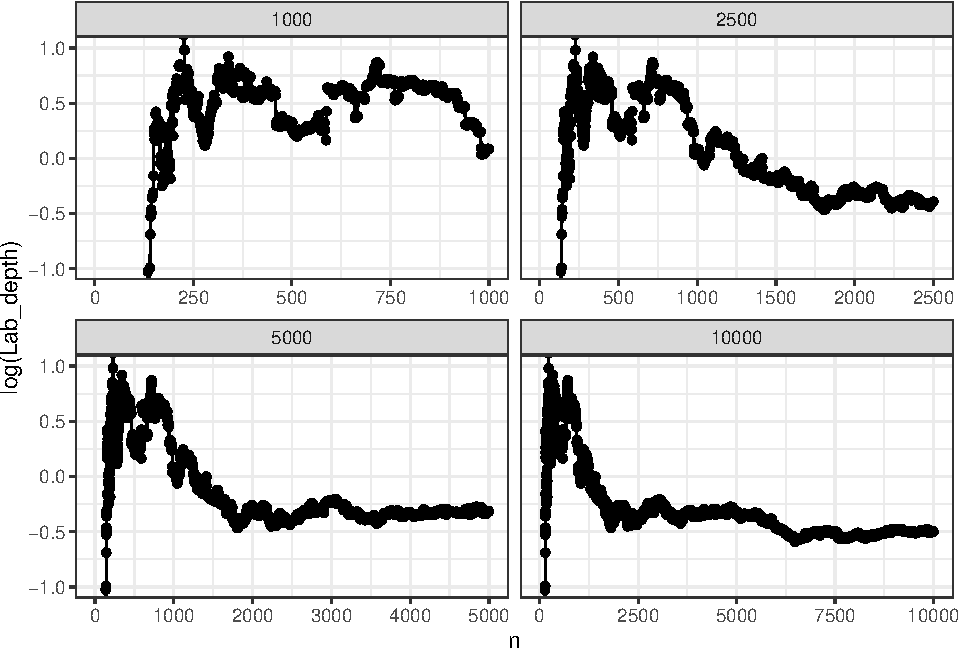
\includegraphics[width=4.5in]{FIGURES/ex2_cvg_plot-1.pdf}
\caption{Convergence by the number of runs.}
\label{Ex_2-convergence_of_mean}
\end{figure}

\hypertarget{discussion}{%
\subsection{Discussion}\label{discussion}}

First we look at the sensitivity of maximum temperature FED in the Foyer. Selected results are displayed in Table  \ref{tbl:Ex_2-1}. The single most significant factor is the depth of the lab space--where the fire occurred. A one-percent change in the lab depth will produce a 0.53~\% decrease in the maximum heat FED for the Foyer. Similarly a one percent change in the height of the Foyer and halls produces a 0.47~\% decrease in the heat FED for the Foyer. At the other end of the scale changes in the Foyer width or the depth of office 1 produce minimal changes to the heat FED for the Foyer

\noindent
\begin{table}[ht]
\begin{center}
\caption[Selected result for sensitivity of maximum temperature FED.]{Selected result for sensitivity of maximum temperature FED.}
\label{tbl:Ex_2-1}
\begingroup
\renewcommand{\arraystretch}{1.2}
\begin{tabular}{@{\extracolsep{\fill}}|l|l|l|l|l|l|}
\hline
\parbox{1.5in}{\bf Variable}    & \parbox{0.75in}{\bf Value}  & \parbox{0.75in}{\bf Std. Error} & \parbox{0.75in}{\bf t value} & \parbox{0.75in}{\bf Pr(\textgreater\textbar t\textbar)} & \parbox{0.75in}{ } \\ \hline
log(Lab\_depth) & -0.5328 & 0.16 & -3.33 & 0.0009 & *** \\
log(Front\_Hall\_depth) & 0.1206 & 0.16 & 0.75 & 0.4551 & \\
log(Foyer\_width) & 0.0053 & 0.16 & 0.03 & 0.9735 & \\
log(\texttt{Office\_\#1\_depth}) & -0.0042 & 0.16 & -0.03 & 0.9791 & \\
log(\texttt{Office\_\#2\_height}) & 0.4525 & 0.16 & 2.84 & 0.0045 & ** \\
log(Foyer\_and\_Halls\_height) & -0.4661 & 0.16 & -2.94 & 0.0033 & ** \\
log(FrontHall2EvenHall\_WIDTH) & -0.0054 & 0.16 & -0.03 & 0.9727 & \\
log(Gyp\_Emissivity.1) & 0.1223 & 0.16 & 0.76 & 0.4458 & \\
log(\texttt{Ofice\_\#4\_\_Door\_Height}) & -0.0029 & 0.16 & -0.02 & 0.9856 & \\
log(\texttt{Ofice\_\#6\_\_Door\_Height}) & 0.1209 & 0.16 & 0.75 & 0.4512 & \\
log(Fire\_HRR\_scaling\_factor) & 0.0398 & 0.16 & 0.25 & 0.8051 & \\
log(Fire\_time\_scaling\_factor) & -0.3920 & 0.16 & -2.45 & 0.0141 & * \\ \hline
\end{tabular}
\endgroup
\end{center}
\end{table}

In Table  \ref{tbl:Ex_2-2}, we look at just those variables for which a one-percent change produces a change of greater than 0.2~\% in the time to non-viability for the Foyer, plus the scaling factors for the fire. Those variables include variables related to the room of fire origin (Lab\_depth), factors related to the space itself (Foyer\_width, Front\_Door\_Width), factors related to the spaces through which the fire must travel (Even\_Hallway\_depth, Odd\_Hallway\_width, Front\_Hall\_depth) and some additional miscellaneous factors (Office\_.2\_height Office\_.5\_height Gyp\_Conductivity.1 Gyp\_Density.1).

\noindent
\begin{table}[ht]
\begin{center}
\caption[Selected results for sensitivity of time to nonviability for Foyer Heat FED.]{Selected results for sensitivity of time to nonviability for Foyer Heat FED.}
\label{tbl:Ex_2-2}
\begingroup
\renewcommand{\arraystretch}{1.2}
\begin{tabular}{@{\extracolsep{\fill}}|l|l|l|l|l|l|}
\hline
\parbox{1.5in}{\bf Variable}    & \parbox{0.75in}{\bf Value}  & \parbox{0.75in}{\bf Std. Error} & \parbox{0.75in}{\bf t value} & \parbox{0.75in}{\bf Pr(\textgreater\textbar t\textbar)} & \parbox{0.75in}{ } \\ \hline
log(Lab\_depth) & 0.3460 & 0.14 & 2.40 & 0.0162 & * \\
log(Even\_Hallway\_depth) & 0.3043 & 0.14 & 2.12 & 0.0341 & * \\
log(Odd\_Hallway\_width) & 0.2359 & 0.14 & 1.64 & 0.1011 & \\
log(Front\_Hall\_depth) & -0.2318 & 0.15 & -1.59 & 0.1116 & \\
log(Foyer\_width) & -0.2778 & 0.15 & -1.91 & 0.0555 & . \\
log(\texttt{Office\_\#2\_height}) & -0.2103 & 0.14 & -1.46 & 0.1431 & \\
log(\texttt{Office\_\#5\_height}) & 0.2564 & 0.14 & 1.78 & 0.0753 & . \\
log(Gyp\_Conductivity.1) & 0.2454 & 0.14 & 1.70 & 0.0889 & . \\
log(Gyp\_Density.1) & 0.2217 & 0.14 & 1.54 & 0.1233 & \\
log(Front\_Door\_Width) & 0.3057 & 0.14 & 2.13 & 0.0333 & * \\
log(Fire\_HRR\_scaling\_factor) & -0.0462 & 0.15 & -0.32 & 0.7510 & \\
log(Fire\_time\_scaling\_factor) & 0.1927 & 0.14 & 1.34 & 0.1790 & \\ \hline
\end{tabular}
\endgroup
\end{center}
\end{table}

%
% -------------------  Summary ------------------------
%

\chapter{Summary and Future Work}

\bibliography{../Bibliography/CFAST_refs}

\appendix
\addcontentsline{toc}{chapter}{Appendices}

%
% -------------------  Nomenclature ------------------------
%

\chapter{Nomenclature}
\label{nomenclature}

Note that the units associated with a given symbol are sometimes changed upon input to and output from the program. In particular, temperatures are typically input in degrees Celsius, converted to Kelvin, and then converted back to Celsius on output. Energy units involving Joules or Watts are typically input as kJ or kW, converted to J or W, then converted back to kJ or kW.

\begin{center}
\begin{longtable}{p{1in}  p{5.5 in}}

$A$                 & area, m$^2$ \\
\end{longtable}

\end{center}

\chapter{PreProcessor Reference}
\label{preprocessor_reference}
Each subsection will discuss one namelist and what each of the parameters does. The tables presented in each subsection are combined in Appendix XXX  to serve as a refence for commands.

\section{Namelist DUMP}

\section{Namelist MHDR}

\section{Namelist MRND}

\section{Namelist MFLD}

\section{Namelist MFIR}

\section {Namelist MSTT}
\chapter{Supplemental Material}

\chapter{Change Log}

\label{last_page}

\end{document}
